\chapter{Diseño e implementación} % Main chapter title

\label{Chapter3} % Change X to a consecutive number; for referencing this chapter elsewhere, use \ref{ChapterX}

\definecolor{mygreen}{rgb}{0,0.6,0}
\definecolor{mygray}{rgb}{0.5,0.5,0.5}
\definecolor{mymauve}{rgb}{0.58,0,0.82}

%%%%%%%%%%%%%%%%%%%%%%%%%%%%%%%%%%%%%%%%%%%%%%%%%%%%%%%%%%%%%%%%%%%%%%%%%%%%%
% parámetros para configurar el formato del código en los entornos lstlisting
%%%%%%%%%%%%%%%%%%%%%%%%%%%%%%%%%%%%%%%%%%%%%%%%%%%%%%%%%%%%%%%%%%%%%%%%%%%%%
\lstset{ %
  backgroundcolor=\color{white},   % choose the background color; you must add \usepackage{color} or \usepackage{xcolor}
  basicstyle=\footnotesize,        % the size of the fonts that are used for the code
  breakatwhitespace=false,         % sets if automatic breaks should only happen at whitespace
  breaklines=true,                 % sets automatic line breaking
  captionpos=b,                    % sets the caption-position to bottom
  commentstyle=\color{mygreen},    % comment style
  deletekeywords={...},            % if you want to delete keywords from the given language
  %escapeinside={\%*}{*)},          % if you want to add LaTeX within your code
  %extendedchars=true,              % lets you use non-ASCII characters; for 8-bits encodings only, does not work with UTF-8
  %frame=single,	                % adds a frame around the code
  keepspaces=true,                 % keeps spaces in text, useful for keeping indentation of code (possibly needs columns=flexible)
  keywordstyle=\color{blue},       % keyword style
  language=[ANSI]C,                % the language of the code
  %otherkeywords={*,...},           % if you want to add more keywords to the set
  numbers=left,                    % where to put the line-numbers; possible values are (none, left, right)
  numbersep=5pt,                   % how far the line-numbers are from the code
  numberstyle=\tiny\color{mygray}, % the style that is used for the line-numbers
  rulecolor=\color{black},         % if not set, the frame-color may be changed on line-breaks within not-black text (e.g. comments (green here))
  showspaces=false,                % show spaces everywhere adding particular underscores; it overrides 'showstringspaces'
  showstringspaces=false,          % underline spaces within strings only
  showtabs=false,                  % show tabs within strings adding particular underscores
  stepnumber=1,                    % the step between two line-numbers. If it's 1, each line will be numbered
  stringstyle=\color{mymauve},     % string literal style
  tabsize=2,	                   % sets default tabsize to 2 spaces
  title=\lstname,                  % show the filename of files included with \lstinputlisting; also try caption instead of title
  morecomment=[s]{/*}{*/}
}

\lstset{literate=
  {á}{{\'a}}1 {é}{{\'e}}1 {í}{{\'i}}1 {ó}{{\'o}}1 {ú}{{\'u}}1
  {Á}{{\'A}}1 {É}{{\'E}}1 {Í}{{\'I}}1 {Ó}{{\'O}}1 {Ú}{{\'U}}1
}

En el presente capítulo se describen el hardware y firmware implementados en el trabajo. Se detalla la integración de los módulos de hardware presentados en el capítulo anterior con el kit ESP32-DevKitC. Luego se presenta el desarrollo del firmware y se fundamentan las decisiones tomadas en el diseño.

%----------------------------------------------------------------------------------------
%	SECTION 1
%----------------------------------------------------------------------------------------
\section{Descripción de hardware}
En esta sección se detalla como se conectaron los diferentes módulos de hardware presentados en el capítulo \ref{Chapter2} con el kit ESP32-DevKitC. Este conexionado se muestra en el diagrama de la figura \ref{fig:conexionado}.

\begin{figure}[htpb]
	\centering
	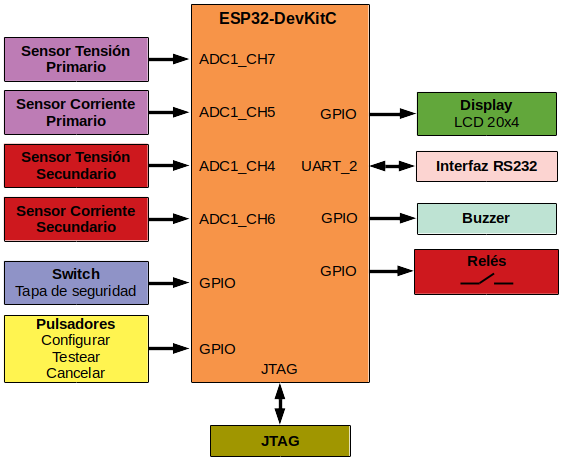
\includegraphics[scale=0.7]{./Figures/diagrama_det.png}
	\caption{Conexionado kit ESP32-DevKitC y módulos de hardware.}
	\label{fig:conexionado}
\end{figure}

Para el conexionado de los elementos del sistema se utilizó una placa universal de 90 mm x 150 mm. Esta permitió un rápido conexionado de los módulos con el kit y la posibilidad de trabajar con hardware y software sin la necesidad de contar con todo el hardware diseñado y construido. En la placa universal se montaron los siguientes componentes:

\begin{itemize}
\item Kit ESP32-DevKitC.
\item Dos fuentes de alimentación de 220 V$_{RMS}$ a 5 V (sección \ref{subsubsec:ModAlim}).
\item El \textit{buzzer}. 
\item Componentes varios necesarios para el apropiado funcionamiento de los módulos analógicos con el kit de desarrollo.
\item Diferentes conectores tipo \textit{header} para el conexionado de los módulos de hardware presentados en el capítulo \ref{Chapter2}.
\end{itemize}

En la tabla \ref{tab:diagramaPines} se muestra el uso de los pines del kit ESP32-DevKitC. En general, todos los módulos fueron conectados directamente al kit con la excepción de los módulos sensores de tensión y corriente cuyo conexionado requirió divisores resistivos para adaptar sus valores de salida al rango de excursión del ADC. A su vez, se incluyó en la placa universal una referencia de tensión basada en el integrado TL431 \citep{TL431}, que se explica con más detalle en la sección \ref{subsec:mejorasAnalo}.

\begin{table}[htpb]
\centering
\caption[Uso de pines del kit ESP32-DevKitC]{Uso de los pines del kit ESP32-DevKitC.}
\begin{tabular}{c c c}
\hline
\toprule
\textbf{Pines kit} & \textbf{Módulo}                        & \textbf{Símbolo}      \\ \hline
\multicolumn{3}{c}{Medición de corrientes y tensiones del transformador}   \\ \hline
IO35/ADC1\_CH7     & Sensor de tensión primario             & PV           \\
IO33/ADC1\_CH5     & Sensor de corriente primario           & PC           \\
IO32/ADC1\_CH4     & Sensor de tensión secundario           & SV           \\
IO34/ADC1\_CH6     & Sensor de corriente secundario         & SC           \\
IO25               & Alimentación bobinado primario         & CPV          \\
IO26               & Alimentación bobinado secundario       & CSV          \\ \hline
\multicolumn{3}{c}{\textit{Display}}                                       \\ \hline
IO18               & \textit{Enable}                        & EN           \\
IO5                & RS                                     & RS           \\
IO19               & \textit{Bus} de datos bit 4            & D4           \\
IO21-23            & \textit{Bus} de datos bits 5 a 7       & D5-7         \\ \hline
\multicolumn{3}{c}{Interfaz RS232}                                         \\ \hline
IO16/RXD2          & Recepción                              & RX           \\
IO17/TXD2          & Transmisión                            & TX           \\ \hline
\multicolumn{3}{c}{Pulsadores}                                             \\ \hline
IO39               & Testear                                & PTEST        \\
IO36               & Configurar                             & PCONF        \\
IO27               & Cancelar                               & PCAN         \\ \hline
\multicolumn{3}{c}{Otros}                                                  \\ \hline
IO4                & \textit{Buzzer}                        & BUZZ         \\
IO2                & \textit{Switch} de seguridad           & SWITCH       \\
IO12-15            & JTAG                                   & -            \\ 
\bottomrule
\hline
\end{tabular}%
\label{tab:diagramaPines}
\end{table}

\subsection{Mejoras a las entradas analógicas}
\label{subsec:mejorasAnalo}
En las secciones \ref{sec:secZMPT101B} y \ref{sec:secZMCT103C} se introdujeron los sensores de tensión y corriente. Estos módulos son muy prácticos debido a que proporcionan valores de tensión acordes para trabajar con el ADC del kit ESP32-DevKitC y, a su vez, proporcionan aislamiento eléctrico de las altas tensiones de los bobinados. Sin embargo, al mirar con más detalle los módulos se pueden identificar las siguientes desventajas:
\begin{enumerate}
\item El amplificador LM358 tiene saturaciones fuertemente asimétricas, V$_{SAT+}$ = Vcc-1,5 V @ Vcc = 5 V y V$_{SAT-} \simeq $  0 V @ Vcc = 5 V. Teniendo en cuenta que el \textit{offset} de salida de los módulos está a la mitad de la alimentación, la saturación positiva limita la excursión de los módulos y por lo tanto, el rango aprovechable del ADC, como se muestra en la figura \ref{fig:sensSat}. 
\item En el caso del sensor de corriente, este no posee \textit{offset} en la salida, esto genera tensiones negativas incompatibles con el ADC del kit.
\item La tensión de alimentación se utiliza como tensión de referencia para generar los 2,5 V de \textit{offset} a la salida del módulo. Si esta tensión no es estable, toda la medición se verá comprometida.
\end{enumerate}

\begin{figure}[htpb]
	\centering
	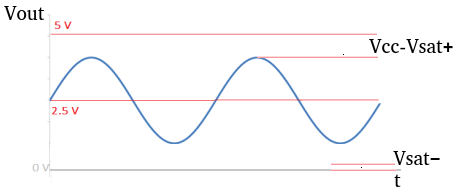
\includegraphics[scale=1]{./Figures/ZMPT101B_waves_sat.png}
	\caption{Saturación módulos sensores.}
	\label{fig:sensSat}
\end{figure}

Luego de estudiar los circuitos se decidió tomar las siguientes acciones para solucionar los problemas encontrados:
\begin{enumerate}
\item Modificar el divisor resistivo que fijaba la tensión de \textit{offset} en la mitad de la alimentación a un valor más acorde, como se muestra en la figura  \ref{fig:sensSatMej}.
\item Eliminar el capacitor de desacople serie a la salida del sensor de corriente. Esto permite que la salida de este módulo excursione solo entre valores positivos.
\item Alimentar los módulos con una referencia de tensión (TL431 \citep{TL431}) en vez de utilizar la tensión de alimentación de la fuente generada en la placa universal.
\end{enumerate}

\begin{figure}[htpb]
	\centering
	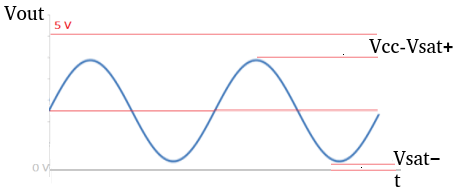
\includegraphics[scale=1]{./Figures/ZMPT101B_waves_sat_mod.png}
	\caption{Saturación mejorada.}
	\label{fig:sensSatMej}
\end{figure}


\subsection{Integración de hardware}

En la figura \ref{fig:gab1} se muestra el trabajo realizado. Como se puede notar, este consta de dos gabinetes, los cuales están conectados por cables que se  observan en la parte derecha de la figura. 

\begin{figure}[htpb]
	\centering
	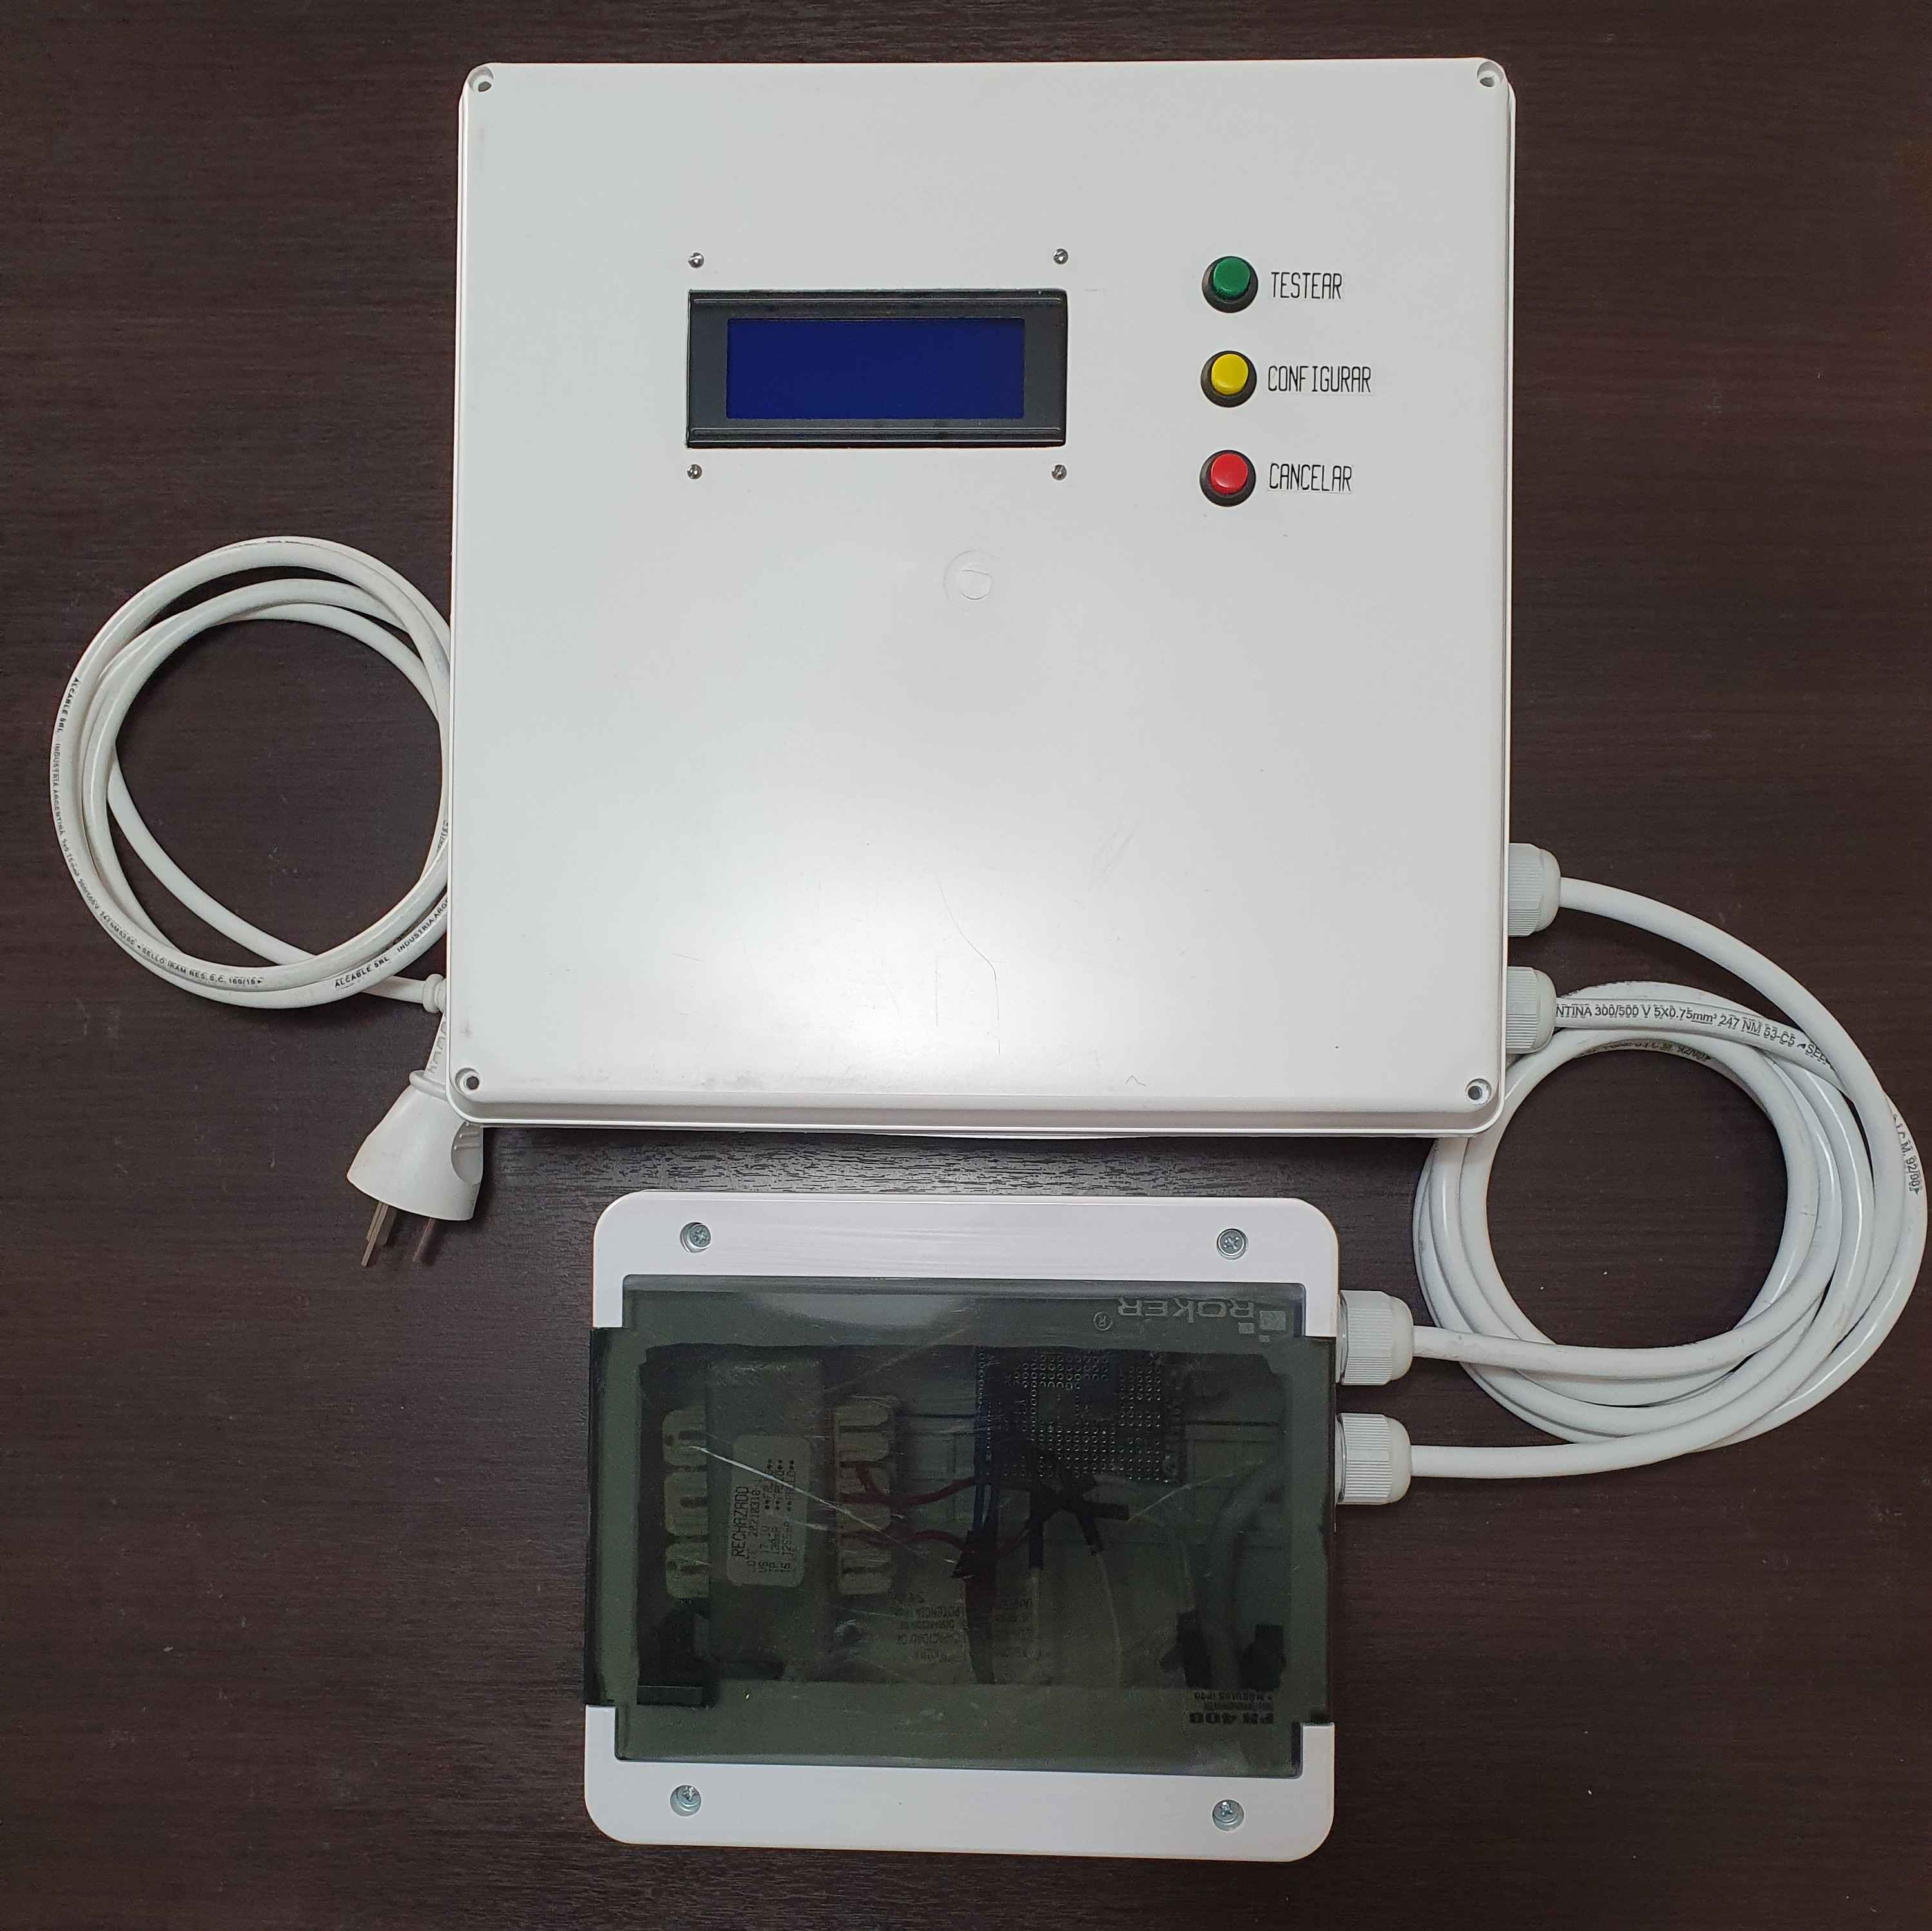
\includegraphics[scale=0.16]{./Figures/gab1.jpg}
	\caption{Trabajo final terminado.}
	\label{fig:gab1}
\end{figure}

En el gabinete de la parte superior de la figura, denominado gabinete principal, se encuentran los diferentes módulos presentados en el capítulo \ref{Chapter2}, los cuales son conectados al kit ESP32-DevKitC a través de la placa universal. Por otro lado, el gabinete de la parte inferior, denominado gabinete auxiliar, está destinado a albergar el transformador que se desea ensayar. En la figura, además, se pueden observar el \textit{display} alfanumérico y los tres pulsadores que fueron rotulados acorde a su función. 

Como se mencionó previamente, en el gabinete auxiliar debe ser colocado el transformador a ensayar. Para esto, cuenta con una tapa gris denominada tapa de seguridad. En la figura \ref{fig:gab2} se muestran los mismos gabinetes con la tapa de seguridad abierta donde se aprecia un transformador de prueba. 

\begin{figure}[h]
	\centering
	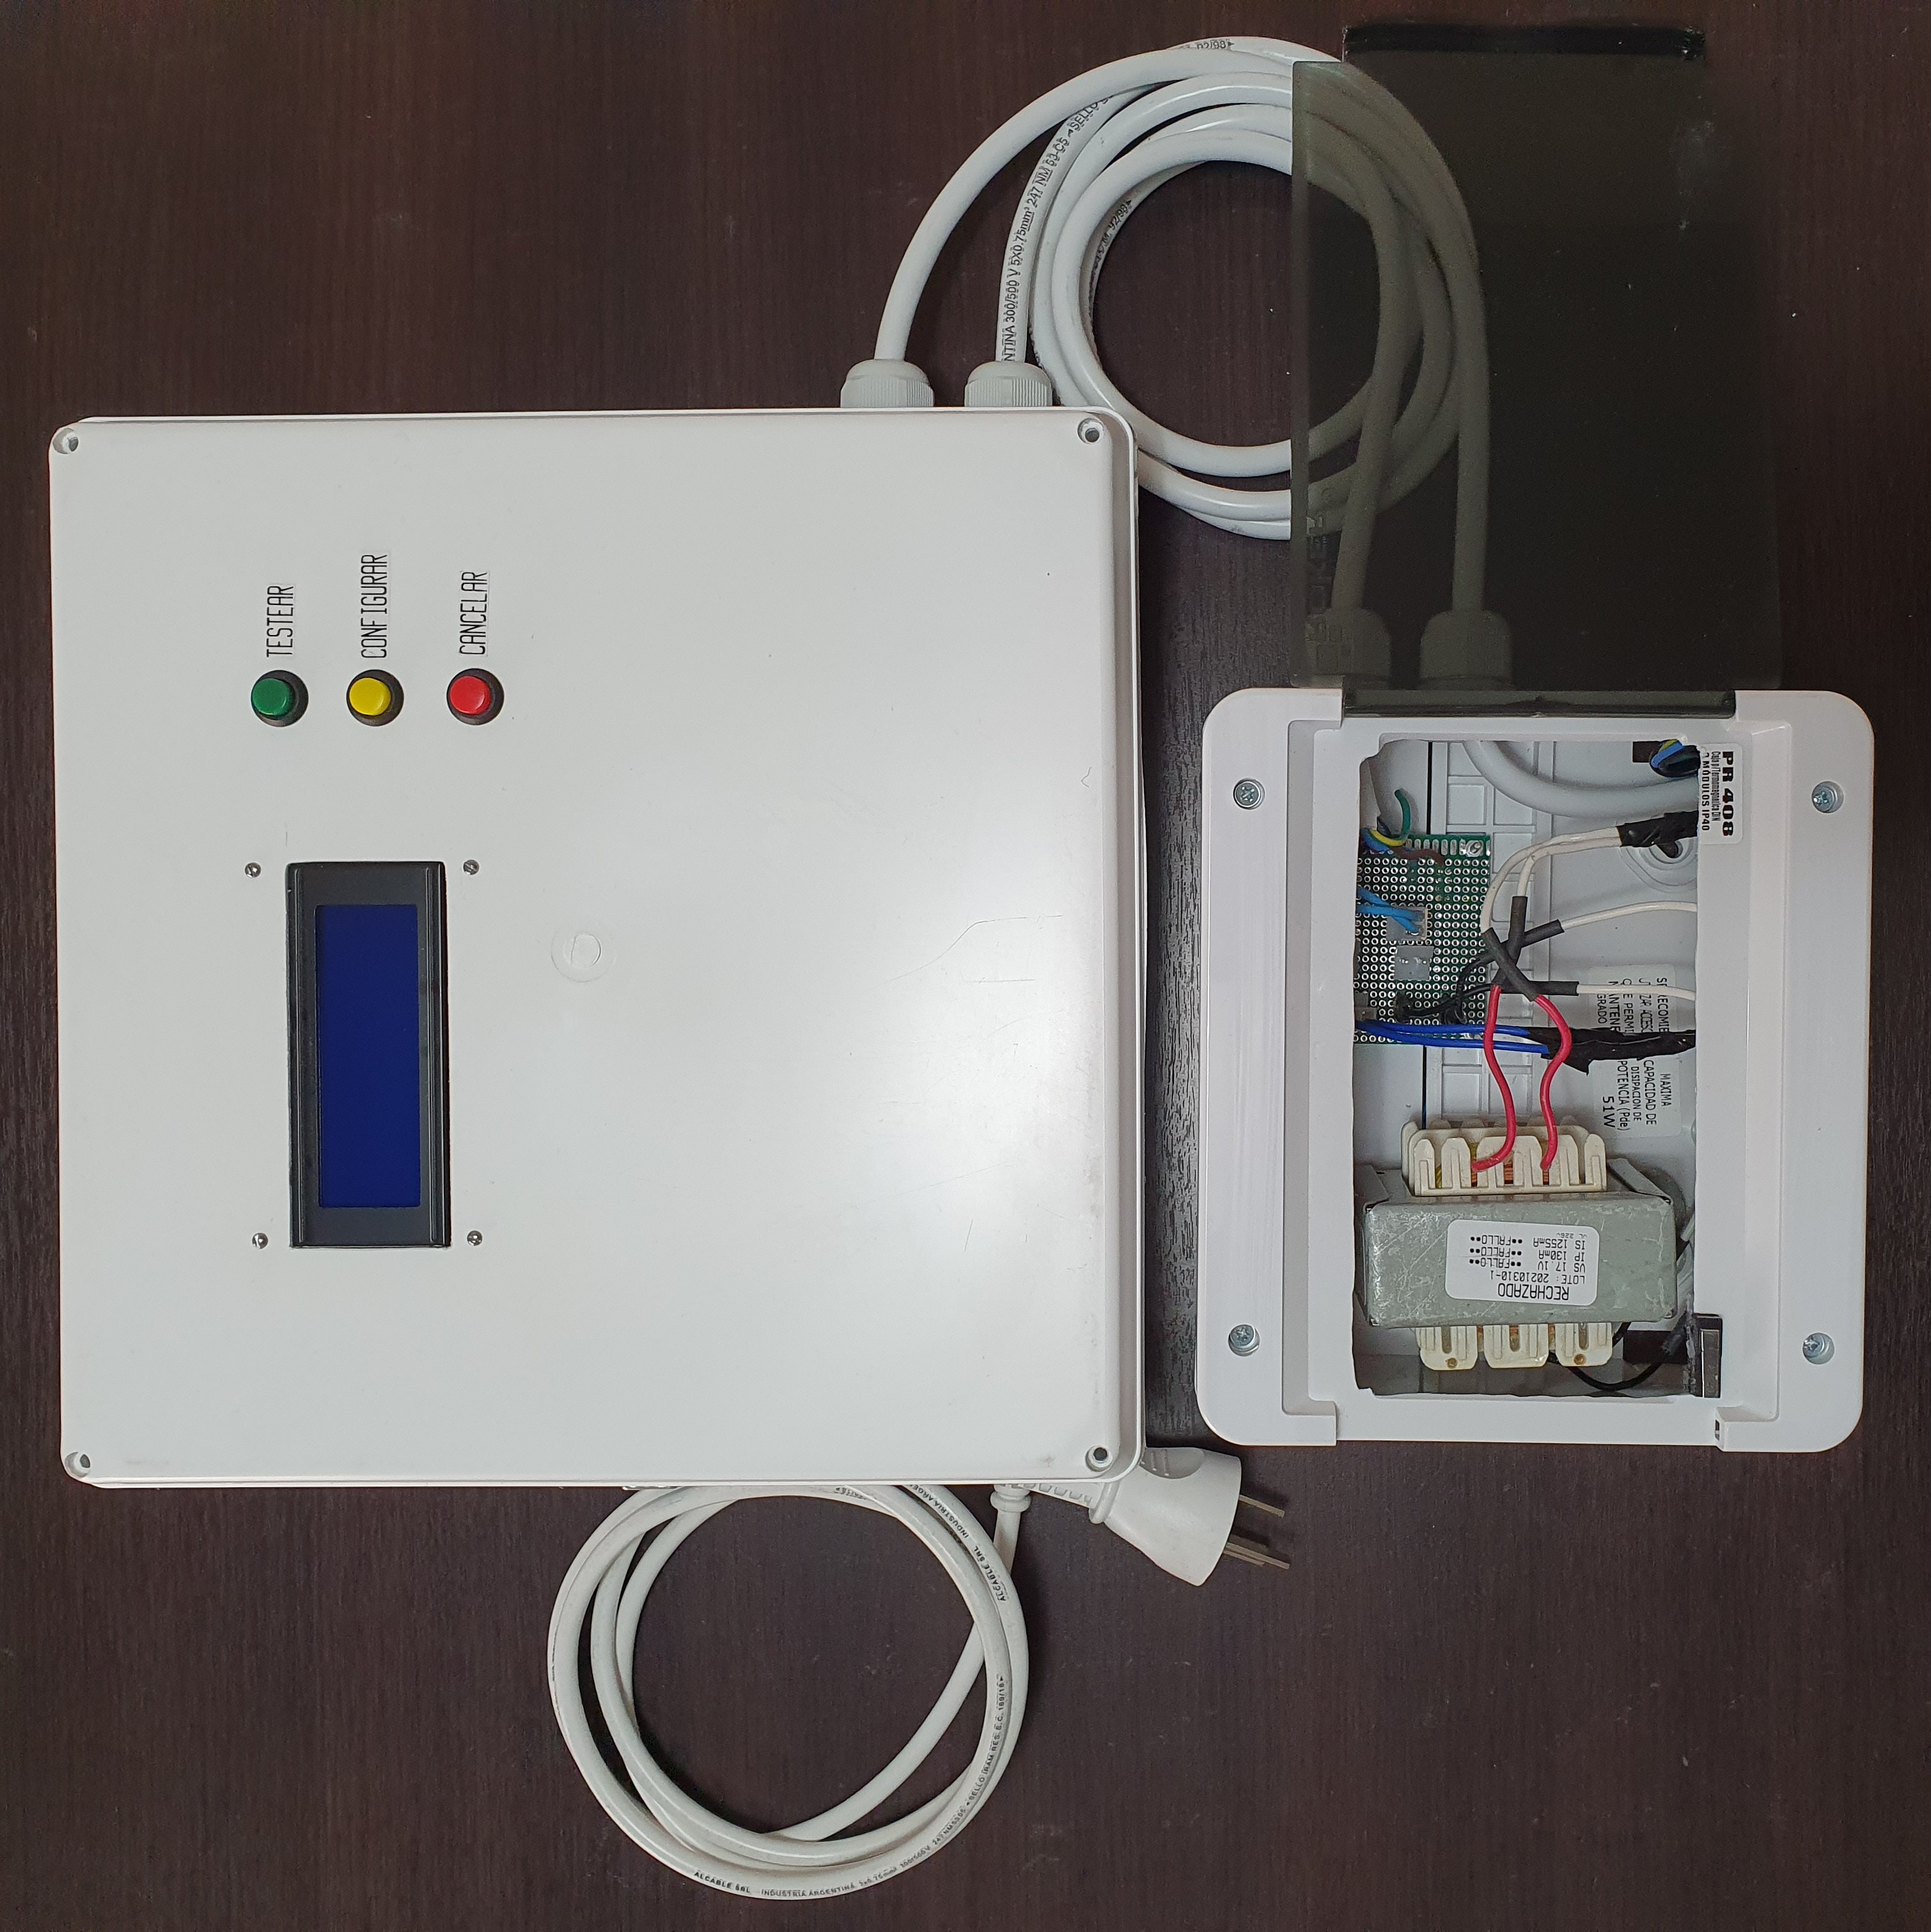
\includegraphics[scale=0.16]{./Figures/gab2.jpg}
	\caption{Trabajo terminado con la tapa de seguridad abierta.}
	\label{fig:gab2}
\end{figure}

\pagebreak

En la figura \ref{fig:gab3} se muestra el gabinete principal sin la tapa. Se pueden distinguir los siguientes componentes:

\begin{itemize}
\item Placa universal con el kit ESP32-DevKitC y componentes asociados.
\item Dos módulos sensores de tensión.
\item Dos módulos sensores de corriente.
\item El módulo de relés.
\item El módulo adaptador RS232.
\item Un transformador que se utiliza como transformador auxiliar para generar la tensión alterna necesaria para alimentar el transformador bajo prueba.
\end{itemize}

Es importante destacar que el armado de los gabinetes fue realizado desde cero con las herramientas disponibles en el hogar y demandó un tiempo considerable. El trabajo terminado, a pesar de ser un prototipo, está en condiciones de ser utilizado como instrumento de medición en un ambiente industrial.

\begin{figure}[h]
	\centering
	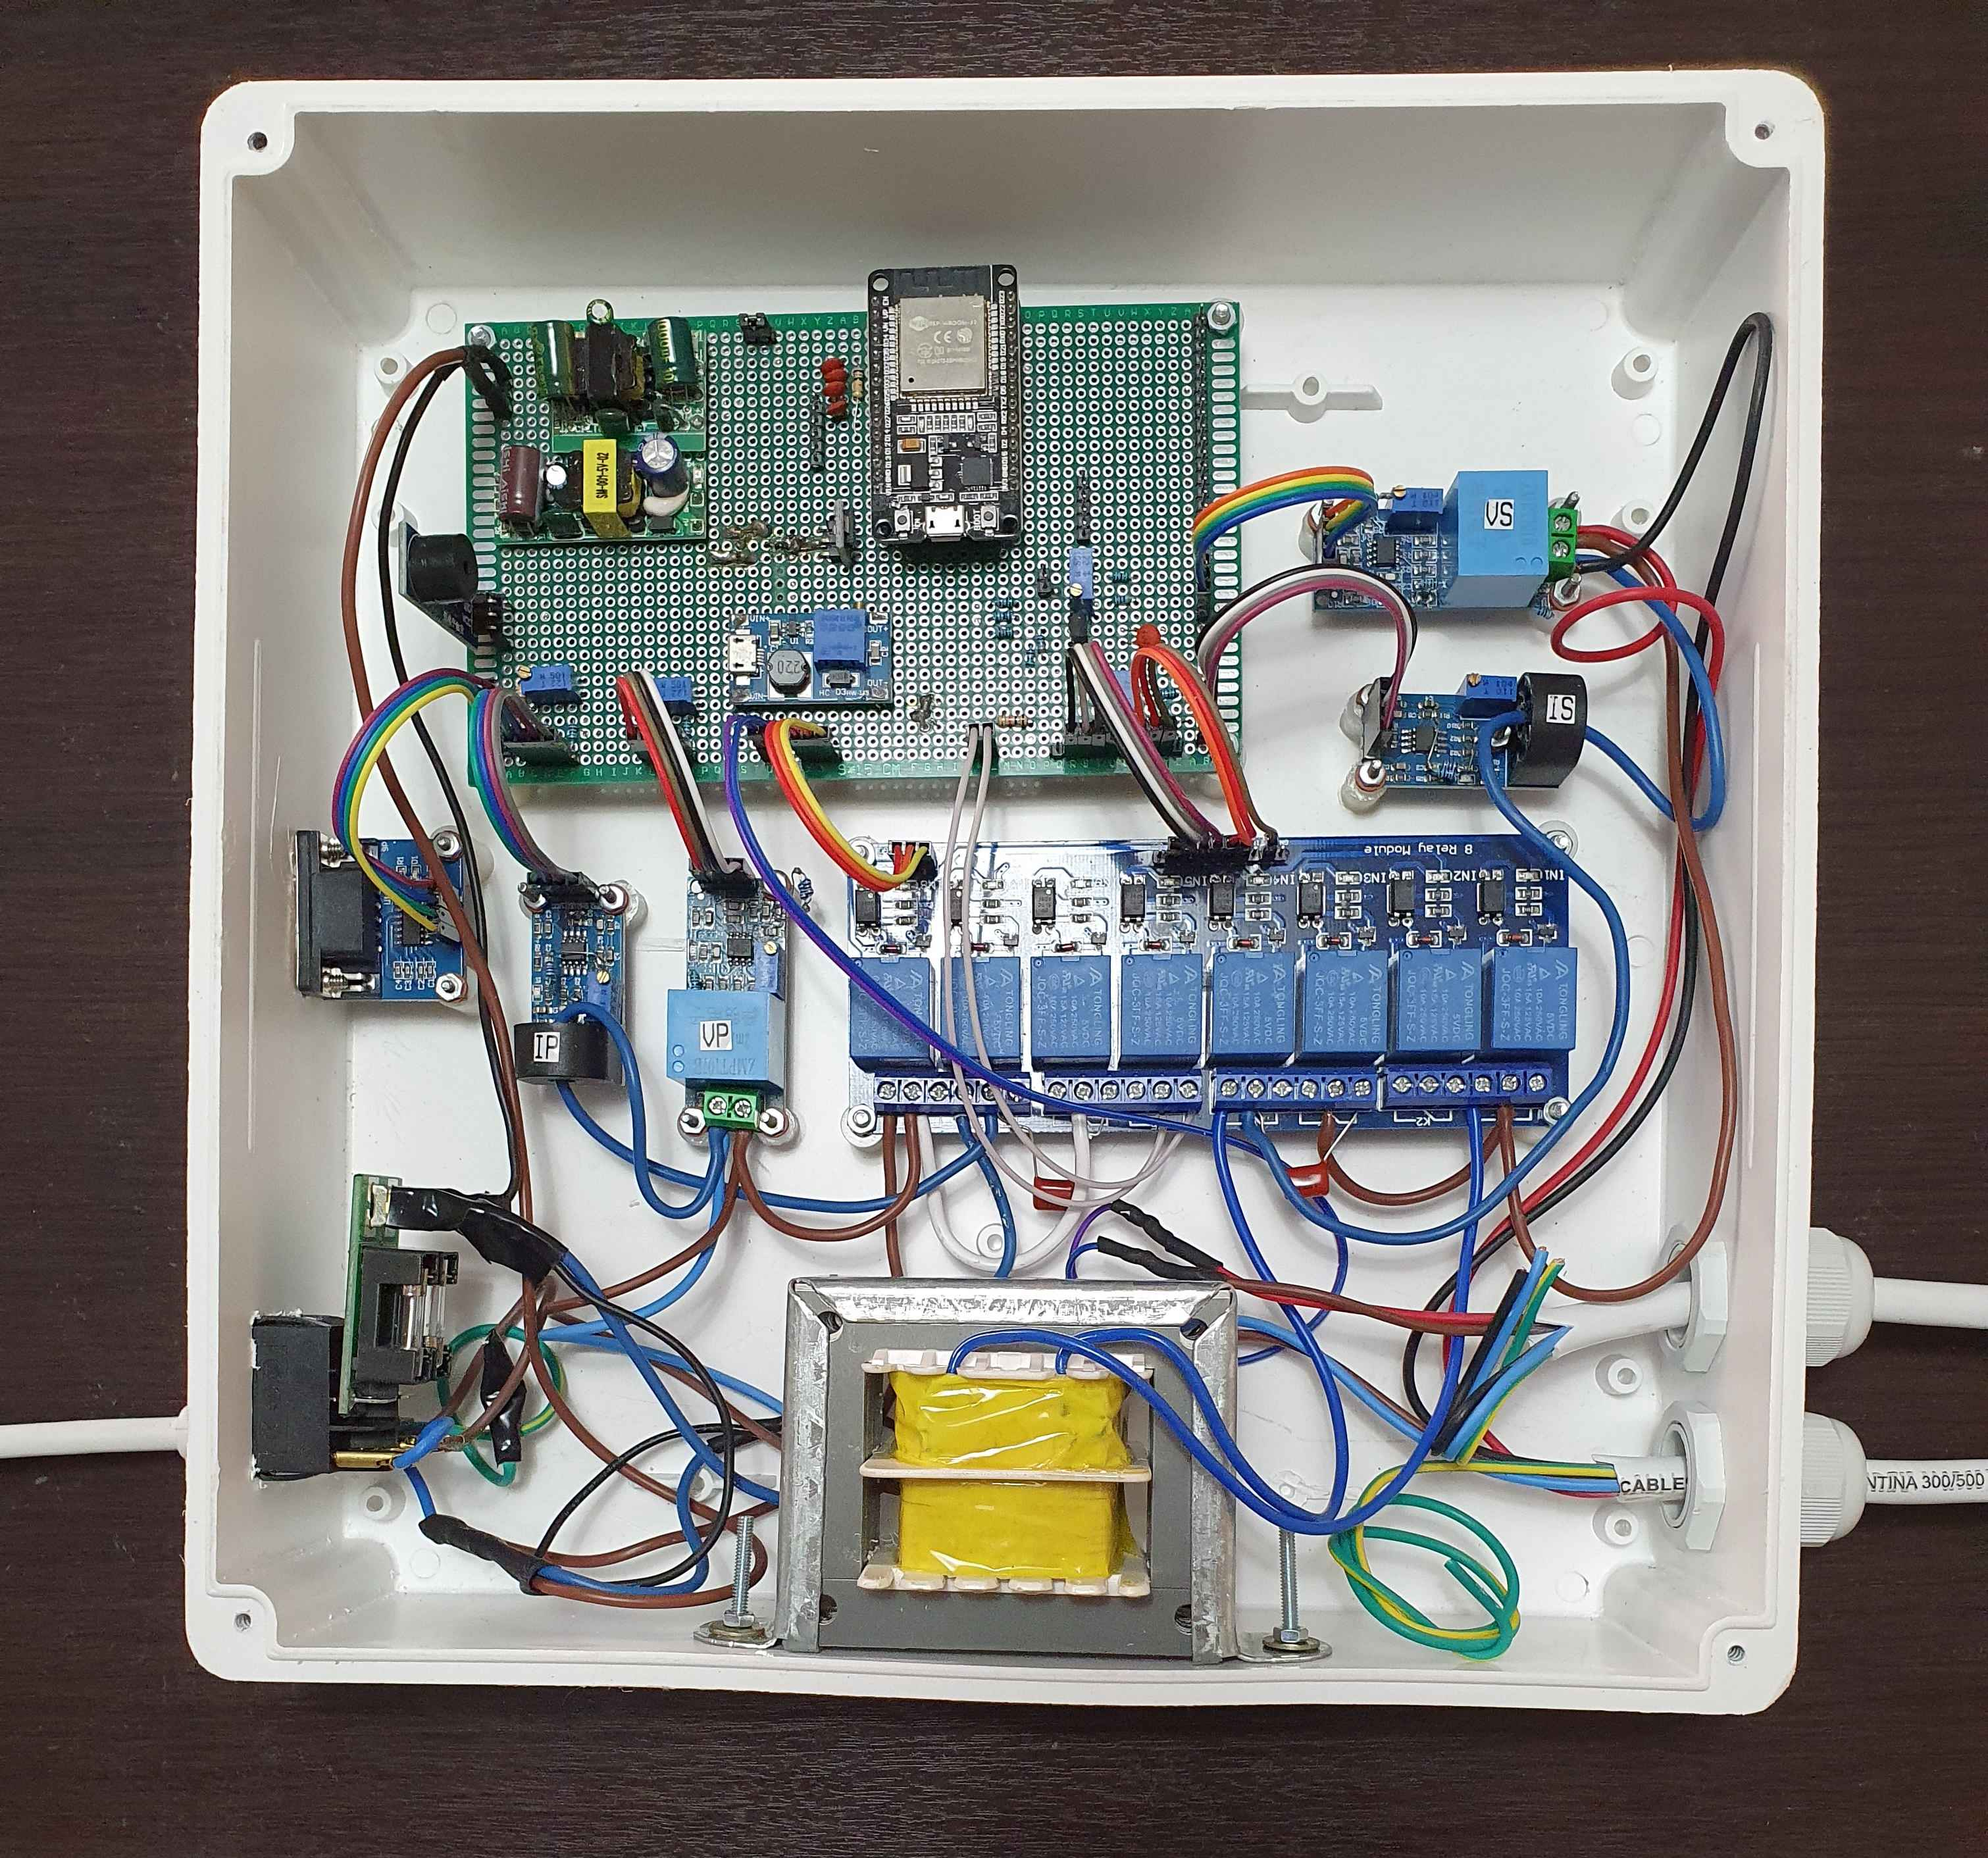
\includegraphics[scale=0.15]{./Figures/gab3.jpg}
	\caption{Contenido gabinete principal.}
	\label{fig:gab3}
\end{figure}

\pagebreak

En la figura \ref{fig:gab4} se muestra el gabinete auxiliar donde se pueden observar los diferentes conectores para el conexionado del transformador a ensayar.

\begin{figure}[hb]
	\centering
	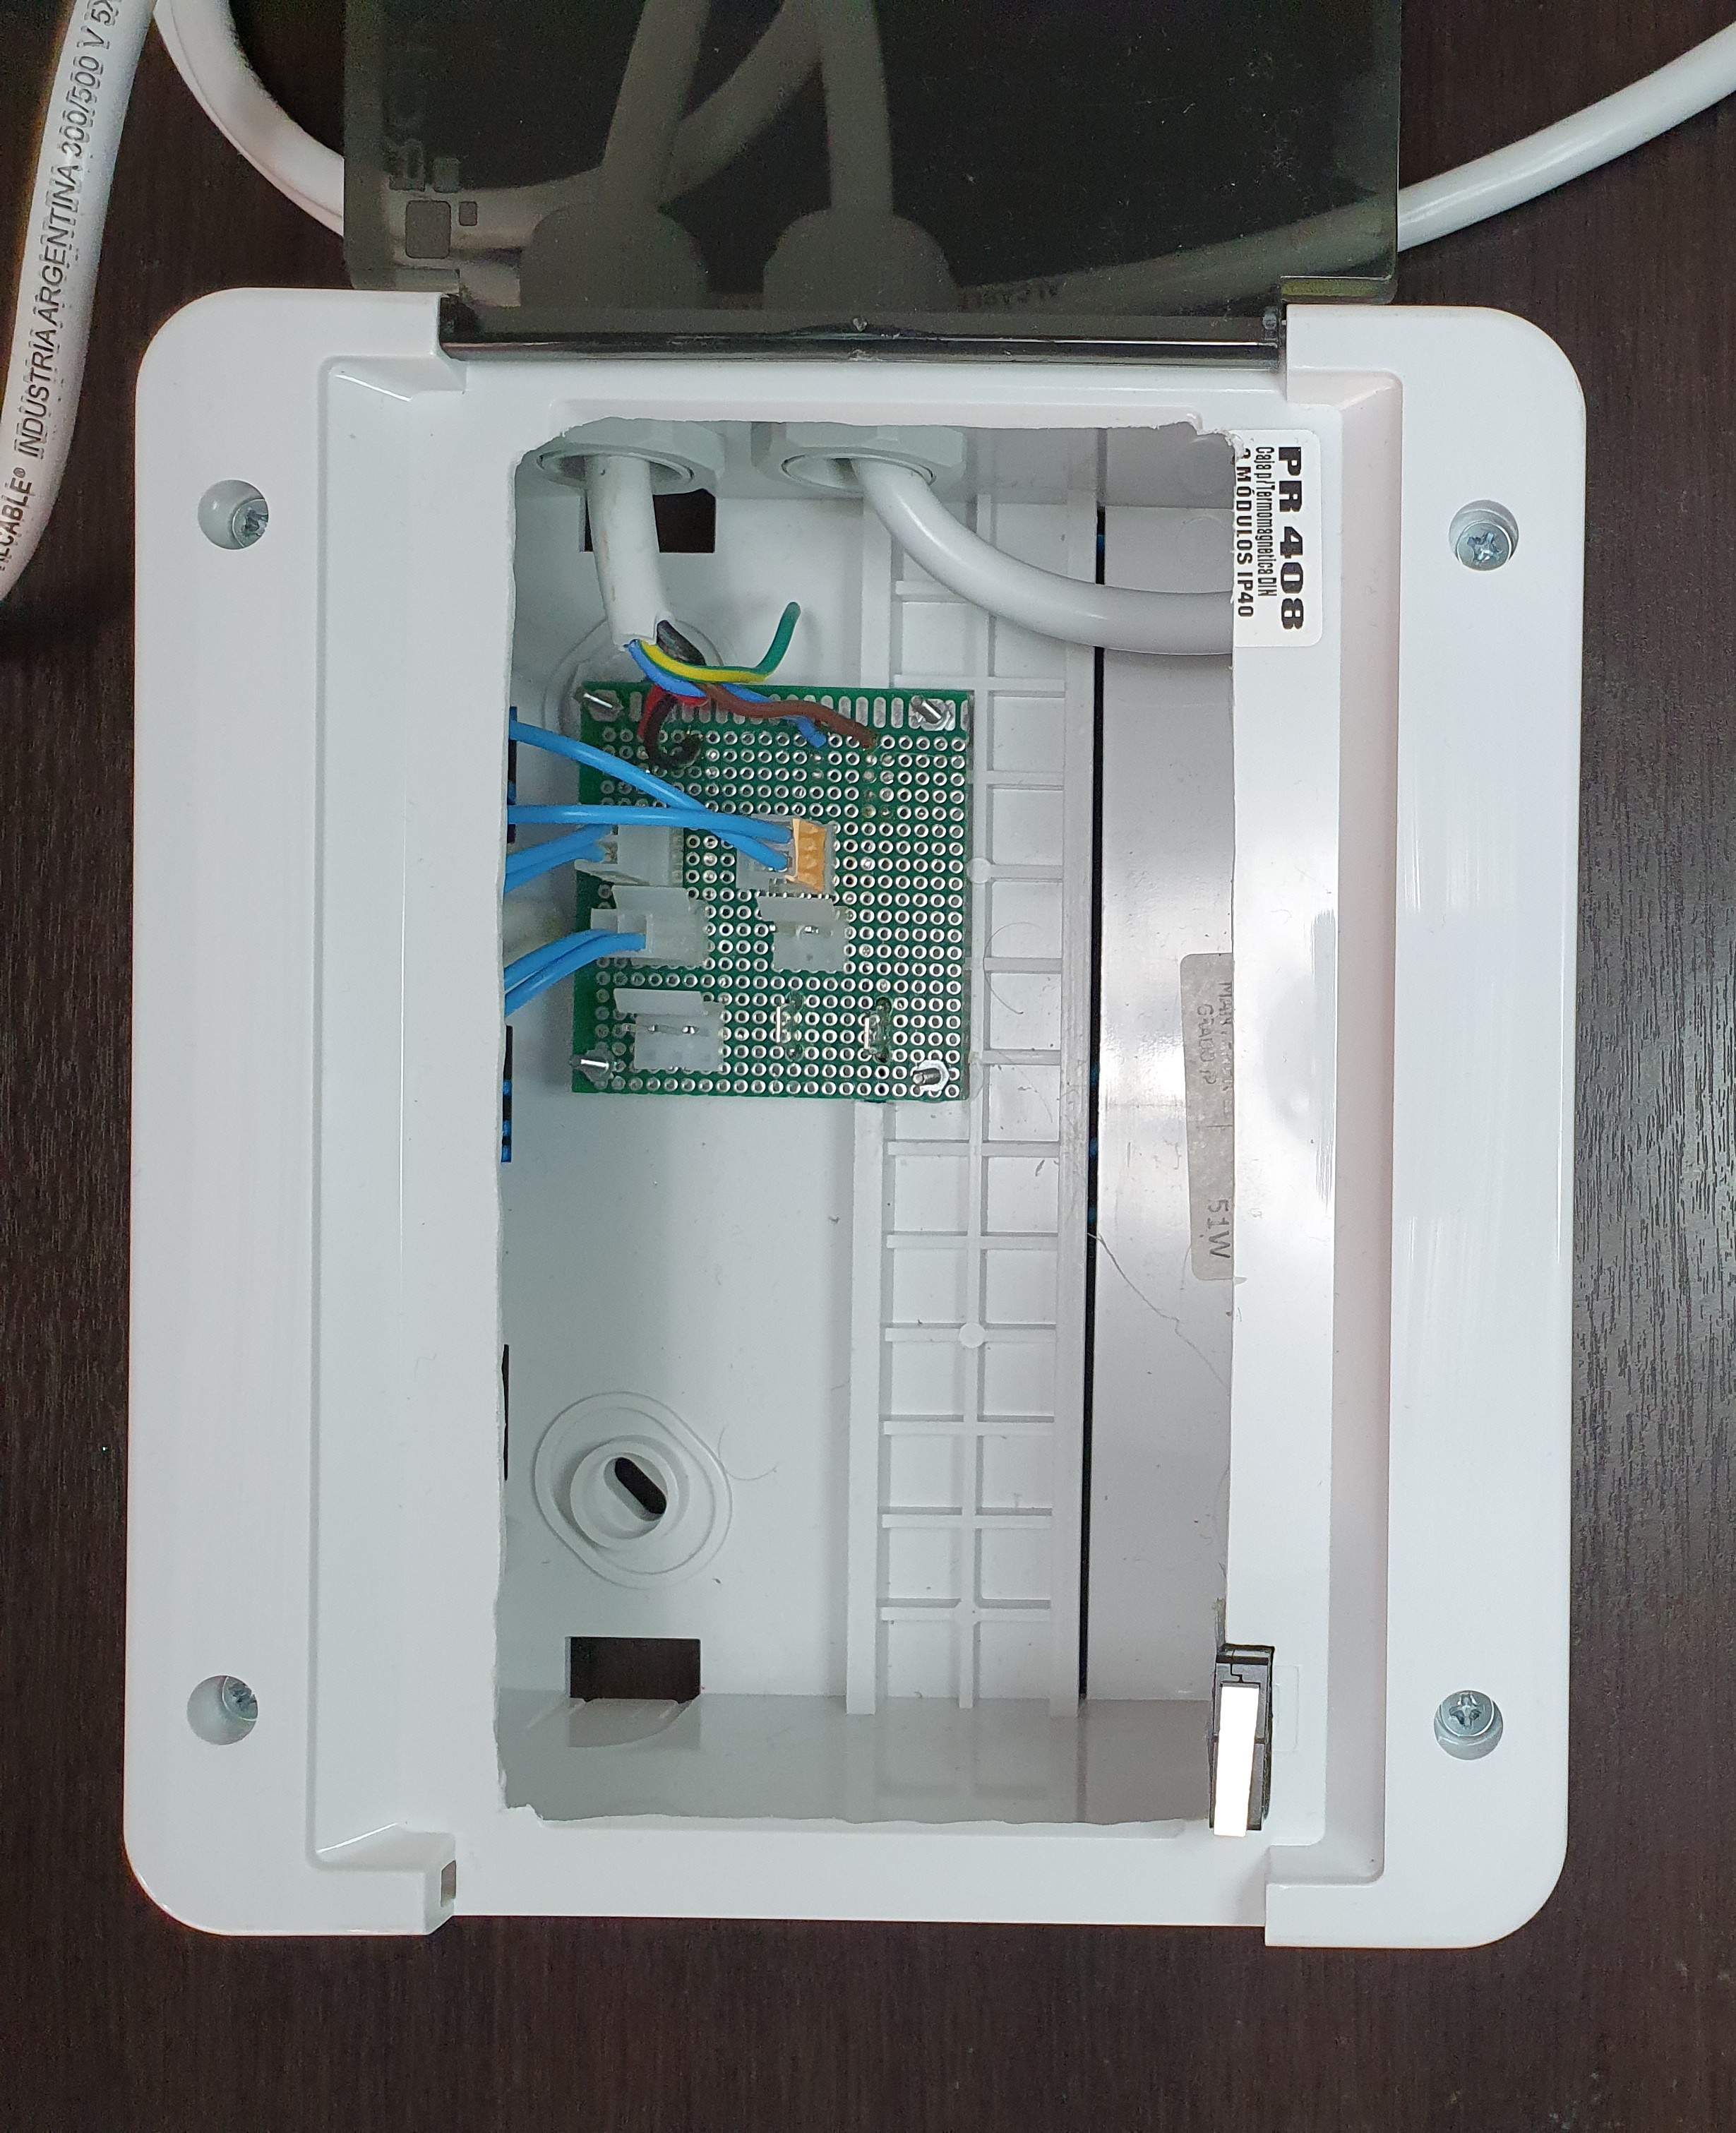
\includegraphics[scale=0.08]{./Figures/gab4.jpg}
	\caption{Gabinete auxiliar sin el transformador a ensayar.}
	\label{fig:gab4}
\end{figure}


\section{Descripción de firmware}

En esta sección se describe la arquitectura de firmware adoptada, así como los módulos principales que la componen, se brinda detalle de las diferentes implementaciones y se destacan sus aspectos más importantes.

\subsection{Arquitectura de firmware}
Luego de analizar posibles patrones de arquitectura de software a utilizar se decidió utilizar el patrón observar y reaccionar visto en Ingeniería de Software \citep{INGSOFT}, que se visualiza en la figura \ref{fig:patron}. Este patrón se utiliza cuando un conjunto de sensores se monitorean y muestran de manera rutinaria.

\begin{figure}[htpb]
	\centering
	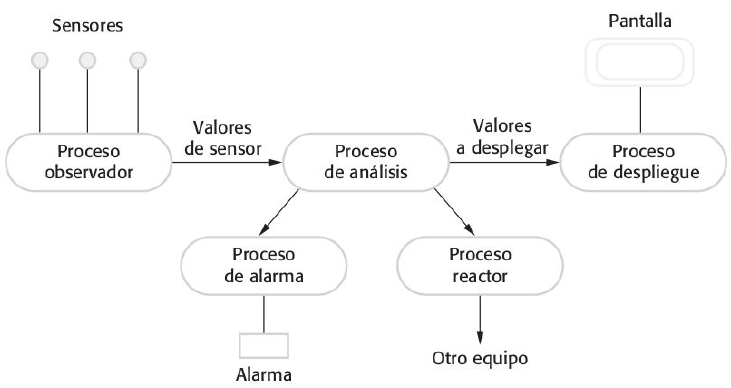
\includegraphics[scale=0.55]{./Figures/patron.png}
	\caption{Patrón observar y reaccionar.}
	\label{fig:patron}
\end{figure}

El dispositivo diseñado responde muy bien a esta arquitectura ya que se deben monitorear los sensores (pulsadores, monitores de tensiones y corrientes), accionar actuadores y enviar los resultados a procesos de salida (\textit{display}, servidor web e impresora). En ningún momento se tienen lazos de realimentación o estructuras que rompan la secuencialidad del sistema. En la figura \ref{fig:patronAplicado} se muestra el patrón aplicado al trabajo.

\begin{figure}[htpb]
	\centering
	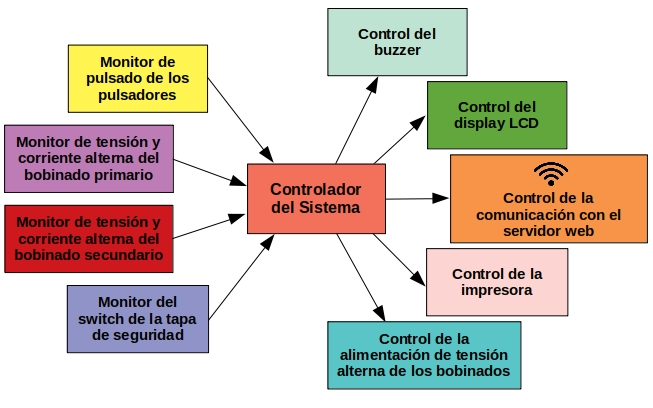
\includegraphics[scale=0.55]{./Figures/arquitecturaSoft.jpg}
	\caption{Patrón observar y reaccionar aplicado al trabajo.}
	\label{fig:patronAplicado}
\end{figure}



\subsection{Estructura general del firmware}

El firmware fue desarrollado por medio de la utilización de buenas prácticas de programación como por ejemplo el control de versiones, la modularización y la documentación del código fuente. Para llevar adelante el control de versiones se creó un repositorio en GitHub \citep{TP_CESE} desde el inicio del trabajo. En cuanto a la modularización, se creó una estructura de módulos y archivos como la siguiente:

\dirtree{%
.1 TP\_CESE.
.2 inc.
.3 app\_adc.h.
.3 app\_Comm.h.
.3 ...
.2 sch.
.2 src.
.3 app\_adc.c.
.3 app\_Comm.c.
.3 ...
.3 main.c.
.3 ...
.2 .gitignore.
.2 CMakeLists.txt.
.2 sdkconfig.
.2 Doxyfile.
.2 README.md.
}

Donde: 
\begin{itemize}
\item inc: directorio para ubicar todos los archivos de cabeceras.
\item sch: directorio con el diagrama esquemático de la placa universal en KiCad \citep{KICAD}.
\item src: directorio para ubicar todos los archivos fuentes.
\item CMakeLists.txt: es el archivo principal que usa CMake para construir el proyecto.
\item sdkconfig: este archivo contiene la configuración de todos los componentes del proyecto (incluido ESP-IDF).
\item Doxyfile: archivo de configuración para generar la documentación a través de Doxygen.
\end{itemize}

A continuación se detallan los principales módulos de software desarrollados desde la perspectiva de su archivo de cabecera:

\begin{itemize}
\item adc.h: implementación del manejo de los ADCs para leer las tensiones y corrientes de los bobinados.
\item app\_Comm.h: se utiliza para ``parsear'' los paquetes HTTP enviados y recibidos desde el servidor web.
\item app\_error.h: se utiliza para definir un criterio de error común frente a las diferentes fallas del sistema.
\item app\_fsm.h: máquina de estados finitos del controlador principal.
\item app\_gpio.h: se utiliza para definir las diferentes funciones para el manejo de entradas-salidas de propósito general como por ejemplo los pulsadores, el comando de alimentación de bobinados, etc.
\item app\_lcd.h: define las rutinas necesarias para escribir mensajes en el \textit{display}.
\item app\_printer.h: implementación del protocolo DPL y manejo del puerto RS-232.
\item app\_WiFi.h: implementación de las diferentes rutinas para el manejo del protocolo Wi-Fi.
\item http\_client.h: implementación de las diferentes rutinas para el manejo del protocolo HTTP.
\item main.h: punto de entrada al firmware que inicializa todos los módulos de hardware.
\item test\_status.h: define diferentes macros y tipos de datos utilizados para almacenar el estado de los ensayos.
\end{itemize}

Por otro lado, se utilizó Doxygen para documentar el código fuente \citep{DOXYGEN}.

\subsection{Controlador de sistema}
\label{sec:ContSist}

Este es el bloque más importante y su función principal es coordinar la interacción de los módulos restantes. Está basado en una máquina de estados finitos (FSM por sus siglas en inglés) que, en función de las variables monitoreadas, actúa sobre las controladas. En la figura \ref{fig:patronAplicado} se puede ver dicha FSM.

Las funciones del bloque se detallan a continuación:

\begin{itemize}
\item Procesar el estado de los pulsadores Testear y Cancelar para iniciar y/o detener la secuencia de caracterización.
\item Procesar el estado del pulsador Configurar para leer los umbrales de validación para el transformador bajo ensayo.
\item Procesar los valores leídos de las tensiones y corrientes de los bobinados primario y secundario.
\item Procesar el estado del \textit{switch} de la tapa de seguridad.
\item Generar el comando para alimentar los bobinados.
\item Generar la información para mostrar en el \textit{display} local.
\item Enviar el estado de la medición al \textit{buzzer} para generar las secuencias de sonidos adecuadas.
\item Enviar o solicitar datos al servidor web.
\end{itemize}

En la figura \ref{fig:MainFSM_red} se muestra un diagrama simplificado del controlador. Los estados fueron enumerados para ayudar en la explicación.

En las siguientes secciones se explica en detalle cada estado y su interacción con los diferentes módulos del sistema. Cabe aclarar que no se abordan detalles tales como los motivos por los cuales falló la comunicación con la impresora o la comunicación Wi-Fi ya que estos son detallados en los capítulos posteriores. Solo se explica como los resultados de los diferentes bloques impactan sobre el funcionamiento del controlador principal.
\pagebreak
\begin{figure}[ht]
	\centering
	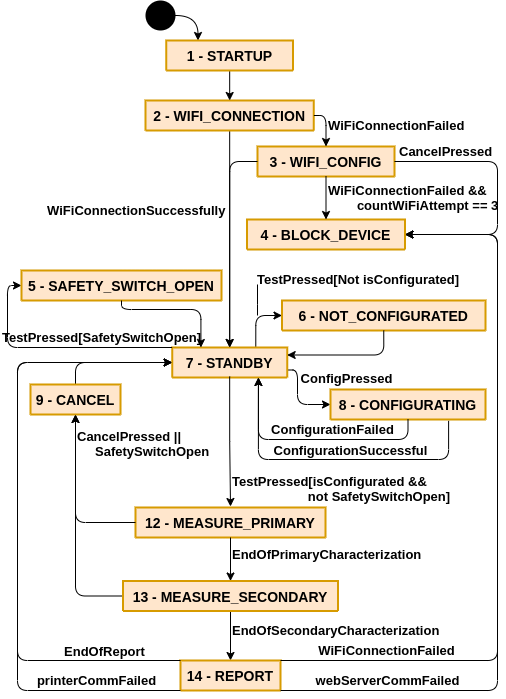
\includegraphics[scale=1]{./Figures/MainFSM_red.png}
	\caption{Diagrama simplificado del controlador del sistema.}
	\label{fig:MainFSM_red}
\end{figure}

Para una mejor explicación se divide a la FSM en diferentes etapas donde cada una agrupa algunos estados:
\begin{itemize}
\item Etapa de inicialización: estados 1, 2 y 3.
\item Etapa de configuración: estados 6, 8, 10 y 11, estos dos últimos no se muestran en la figura \ref{fig:MainFSM_red} por claridad.
\item Etapa de caracterización: estados 5, 9, 12, 13 y 14. 
\item Etapa de reporte: estado 14.
\end{itemize}

Los estados 7 (\textit{STANDBY}) y 4 (\textit{BLOCK\_DEVICE}) se consideran estados particulares y aparecen en todas o casi todas las etapas presentadas. Estos estados se consideran inicio y/o fin de las diferentes etapas.

El estado 14 corresponde al estado de reporte y para mayor claridad, el análisis de dicho estado se dividió en la etapa de caracterización y en la etapa de reporte. En la etapa de caracterización se considera que el reporte fue exitoso, es decir, se pudo imprimir la etiqueta y se pudo mandar la información al servidor web, mientras que en la etapa de reporte se consideran posibles fallas en estas acciones.

\subsubsection{Etapa de inicialización}
\label{subsubsec:EtIni}
En la figura \ref{fig:MainFSM_1} se muestra la sub-máquina de estado correspondiente a la etapa de inicialización. 

Esta etapa se inicia cuando el equipo es energizado (salida de \textit{reset}) y termina en el estado 7 (\textit{STANDBY}) si el equipo fue exitoso al conectarse a Wi-Fi o en el estado  4 (\textit{BLOCK\_DEVICE}) si los intentos de conexión fallaron. 

Luego de la salida de \textit{reset} del sistema y de inicializar todos los módulos de hardware se ingresa en el estado 1 (\textit{STARTUP}). Este estado tiene como función inicializar cuestiones de la máquina de estados principal como la alimentación de bobinados, mostrar un mensaje de bienvenida en el \textit{display} durante un tiempo fijo (\textit{LCD\_MSG\_WAIT}) y limpiar la variable \textit{isConfigurated}. Esta última se utiliza para indicar si el equipo fue configurado. Al iniciar el sistema el equipo no se encuentra configurado.

Luego de transcurrido el tiempo \textit{LCD\_MSG\_WAIT} se transiciona al estado 2 (\textit{WIFI\_CONNECTION}). En este estado se leen los valores SSID y la contraseña desde la memoria no volátil del dispositivo y se intenta conectar a la red Wi-Fi configurada. En caso de fallar la conexión se genera el evento \textit{WiFiConnectionFailed} y se transciona hacia el estado 3 (\textit{WIFI\_CONFIG}). 

En el estado \textit{WIFI\_CONFIG} se consulta si se desea reconfigurar las credenciales de Wi-Fi, para lo cual el operador puede acceder al pulsar Configurar o negarse al pulsar Cancelar. En caso de reconfigurar se utiliza la aplicación ESP-Touch vista en la sección \ref{sec:ESPTouch}, se realizan 3 intentos de reconexión y en caso de fallar nuevamente el equipo pasa al estado 4 (\textit{BLOCK\_DEVICE}) y finaliza la secuencia de inicio.

En caso de lograr la conexión Wi-Fi sea en el estado 2 (\textit{WIFI\_CONNECTION}) o el pseudoestado 3 (\textit{WIFI\_CONFIG}), el sistema pasa al estado 7 (\textit{STANDBY}) y finaliza la secuencia de inicio.

\pagebreak

\begin{figure}[ht]
	\centering
	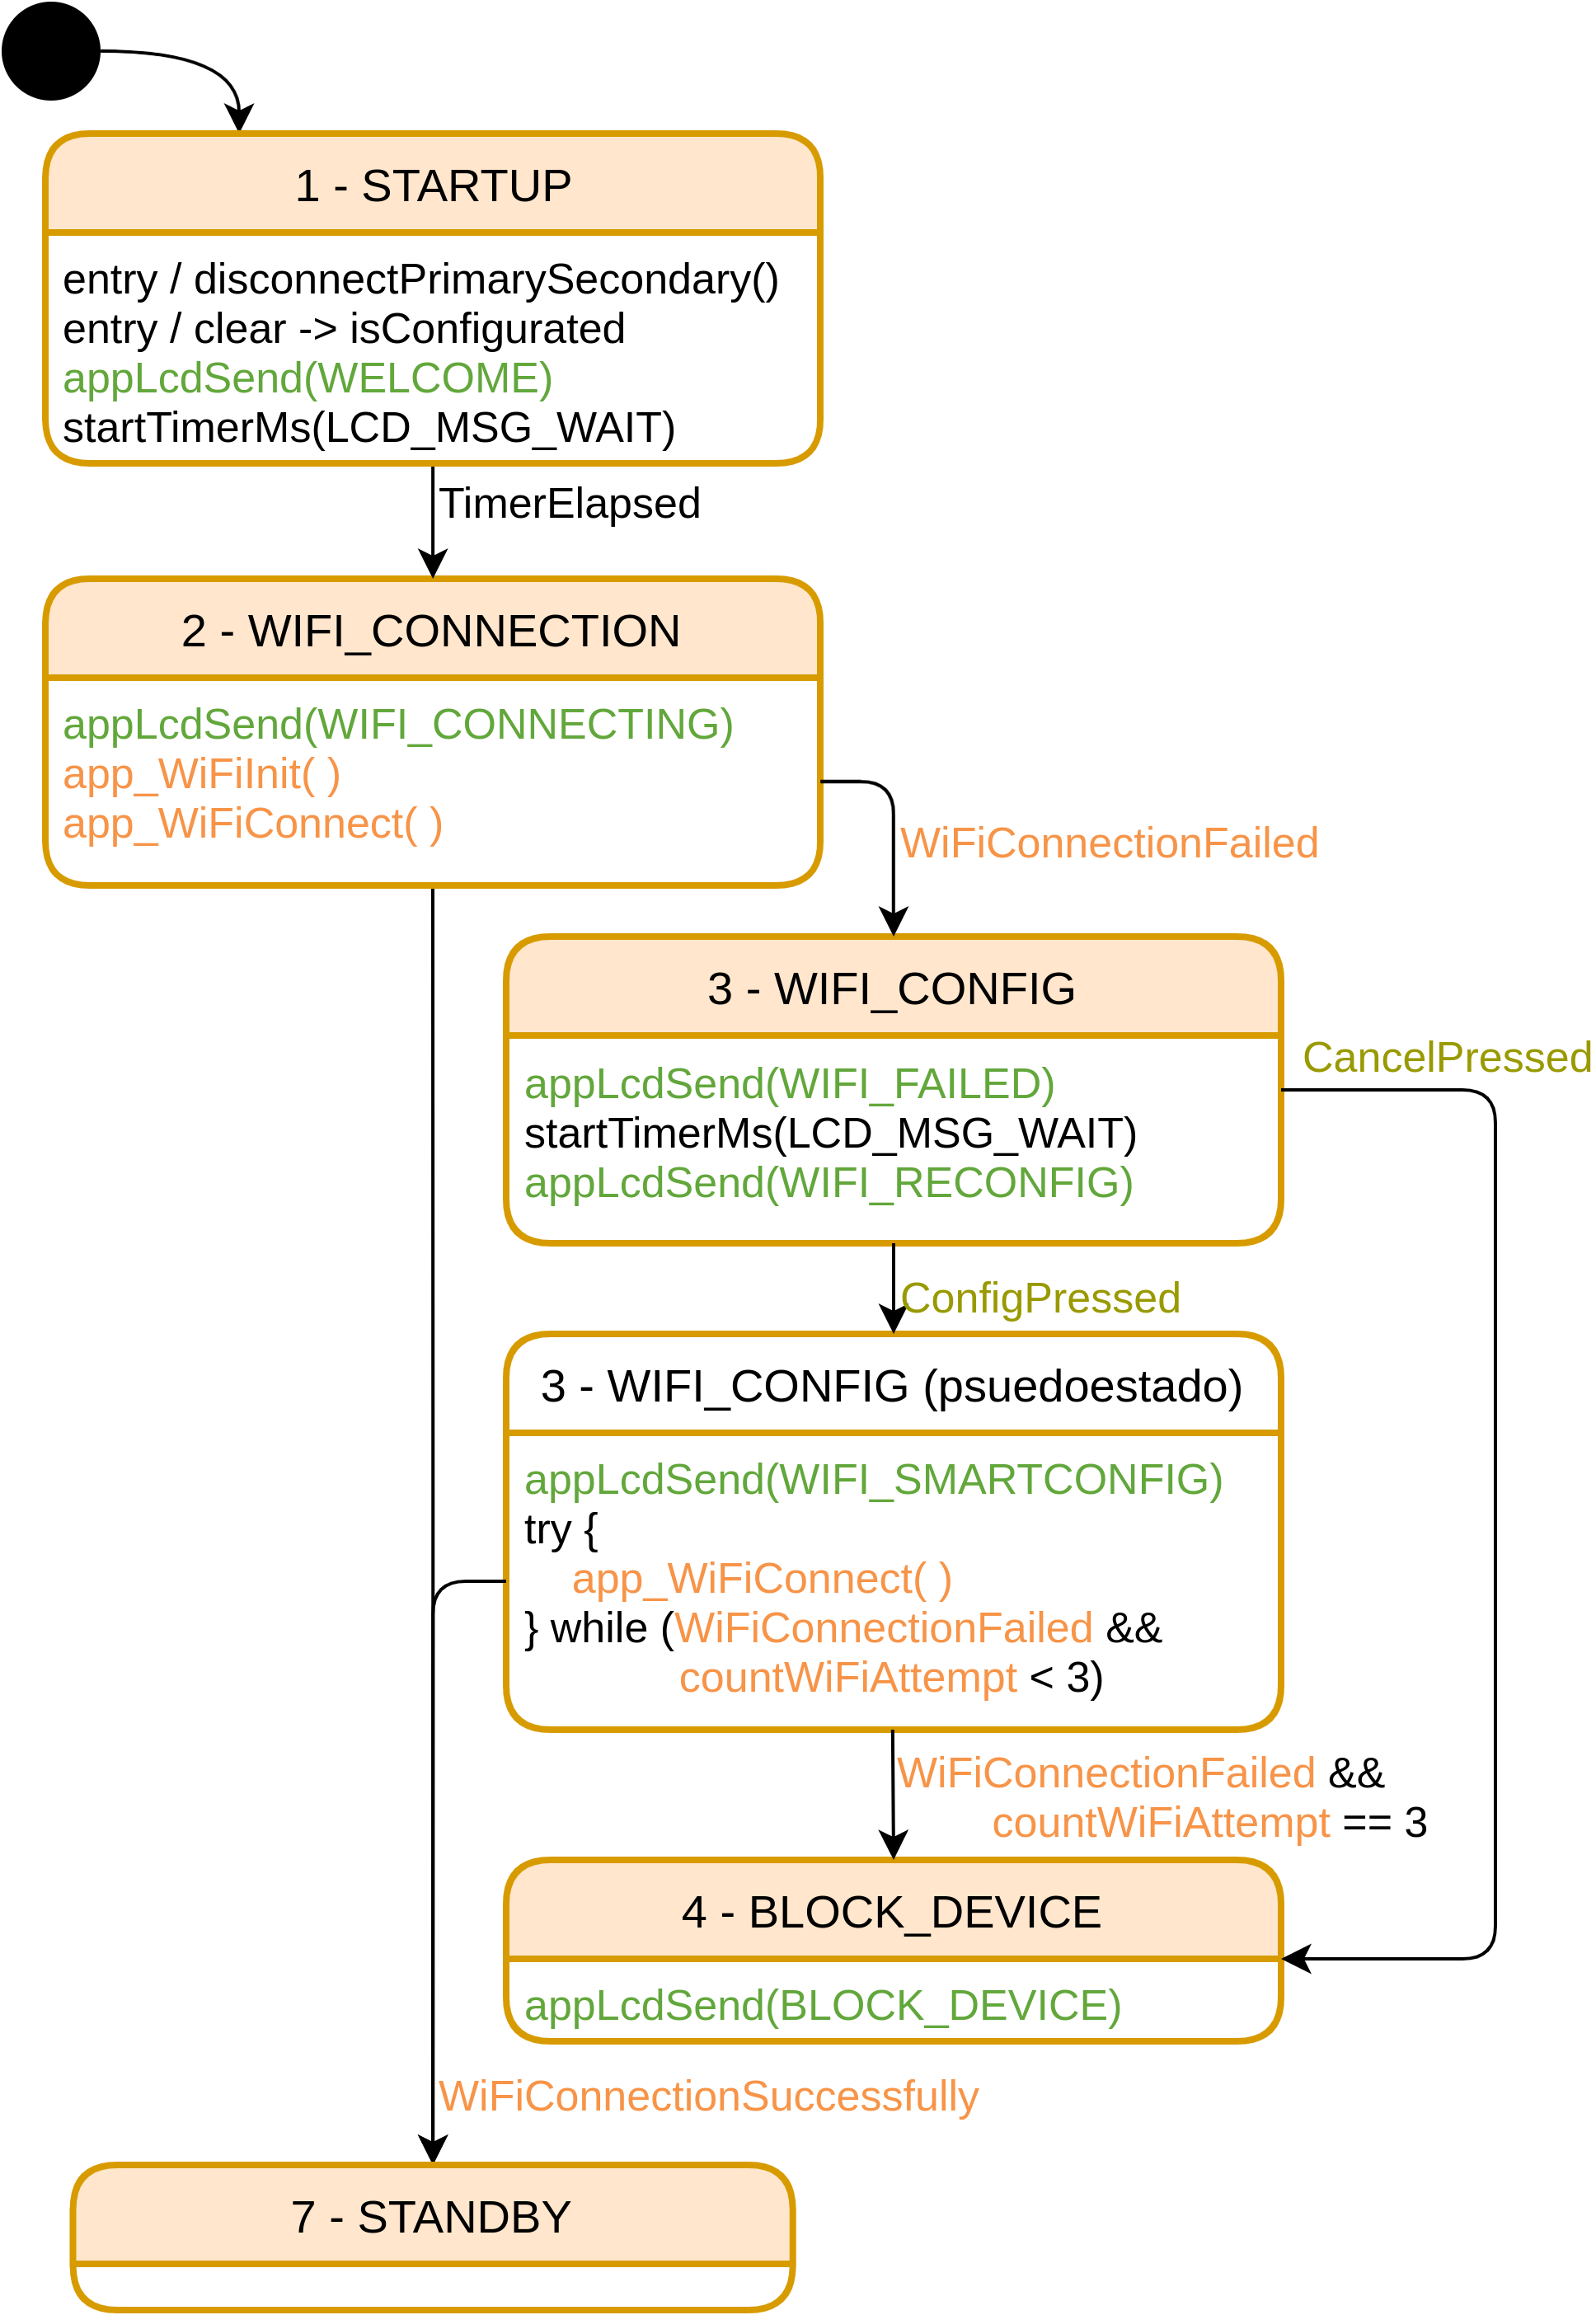
\includegraphics[scale=1]{./Figures/MainFSM_1.png}
	\caption{Etapa de inicialización.}
	\label{fig:MainFSM_1}
\end{figure}


\subsubsection{Etapa de configuración}
\label{subsubsec:EtConf}
En la figura \ref{fig:MainFSM_2} se muestra la sub-máquina de estados correspondiente a la etapa de configuración. 

Luego de la etapa de inicialización se ingresa en la etapa de configuración. Esta etapa se inicia y finaliza en el estado 7 (\textit{STANDBY}) y tiene dos funciones principales:

\begin{itemize}
\item Validar si el equipo fue configurado por medio de \textit{isConfigurated} para permitir pasar a la etapa de caracterización.
\item Pedir los datos de configuración al servidor web al pulsar Configurar y fijar el valor de \textit{isConfigurated} acorde al resultado de dicha acción.
\end{itemize}



\begin{figure}[ht]
	\centering
	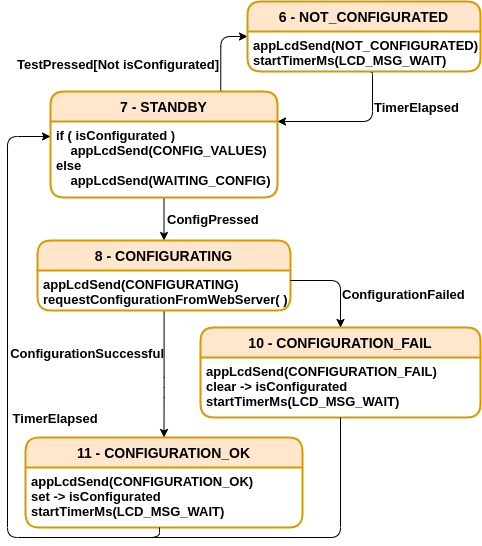
\includegraphics[scale=1]{./Figures/MainFSM_2.png}
	\caption{Etapa de configuración.}
	\label{fig:MainFSM_2}
\end{figure}

En el estado 7 (\textit{STANDBY}) se muestra en el \textit{display} si el equipo fue o no configurado previamente en base al valor de \textit{isConfigurated}. Si el operario desea testear un transformador, para lo cual pulsa Testear, pero la variable \textit{isConfigurated} es cero, el equipo pasa al estado 6 (\textit{NOT\_CONFIGURATED}), muestra un mensaje de equipo no configurado y vuelve al estado \textit{STANDBY}.

Si el operario desea configurar el equipo debe pulsar Configurar, para lo cual se pasa del estado \textit{STANDBY} al estado 8 (\textit{CONFIGURATING}). En este estado se solicitan los valores de configuración al servidor web desarrollado por el cliente. De aquí, se pueden generar dos eventos posibles \textit{ConfigurationSuccessful} o \textit{ConfigurationFailed} que dependen de la obtención de los datos con o sin errores desde el servidor web. En ambos casos se asigna el valor correcto a la variable \textit{isConfigurated} y se muestra en el \textit{display} el resultado.

\subsubsection{Etapa de caracterización}
\label{subsubsec:EtTest}
En la figura \ref{fig:MainFSM_3} se muestra la sub-máquina de estados correspondiente a la etapa de caracterización. 

\begin{figure}[ht]
	\centering
	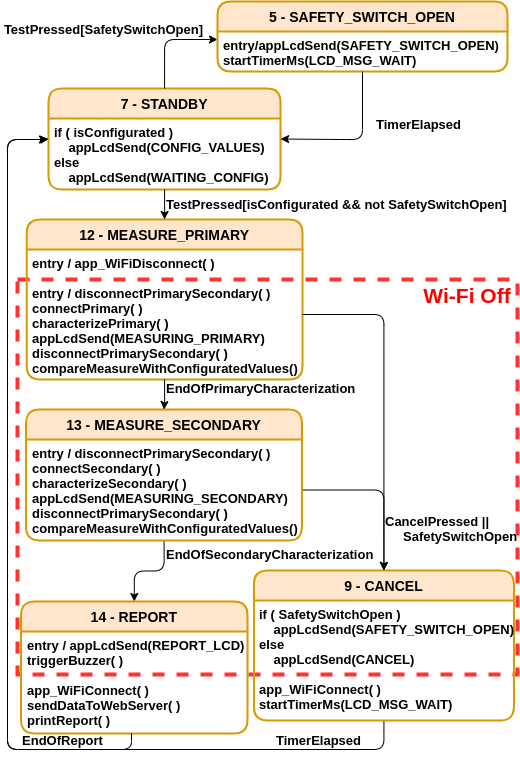
\includegraphics[scale=0.95]{./Figures/MainFSM_3.png}
	\caption{Etapa de caracterización.}
	\label{fig:MainFSM_3}
\end{figure}

Luego de la etapa de configuración se ingresa en la etapa de caracterización. Esta etapa se inicia y finaliza en el estado 7 (\textit{STANDBY}) y tiene varias funciones:

\begin{itemize}
\item Iniciar y procesar los valores leídos de las tensiones y corrientes de los bobinados primario y secundario.
\item Alimentar los bobinados.
\item Determinar los resultados del ensayo para ser reportados en la etapa de reporte.
\item Monitorear en todo momento el \textit{switch} de la tapa de seguridad y evitar o cancelar el proceso de caracterización.
\end{itemize}

Al igual que en la etapa de configuración, en el estado 7 (\textit{STANDBY}) se muestra en el \textit{display} si el equipo fue o no configurado previamente. Se supone que para iniciar la etapa de caracterización el equipo fue configurado, de lo contrario, no se podrá avanzar en la caracterización (estado \textit{NOT\_CONFIGURATED}).

Existen dos caminos posibles en la etapa de caracterización para salir del estado \textit{STANDBY}, ambos son por medio del pulsador Testear, y la diferencia radica en el estado del \textit{switch} de la tapa de seguridad (\textit{SafetySwitchOpen}). Para poder inicializar la caracterización el \textit{switch} debe estar cerrado, en caso contrario, el equipo pasa al estado 5 (\textit{SAFETY\_SWITCH\_OPEN}), muestra un mensaje de tapa de seguridad abierta y vuelve al estado \textit{STANDBY}.

Por otro lado, si al pulsar Testear el \textit{switch} se encuentra cerrado la secuencia de caracterización comenzará normalmente. A continuación se pasa a los estados 12 (\textit{MEASURE\_PRIMARY}) y 13 (\textit{MEASURE\_SECONDARY}). Estos estados fueron simplificados por claridad en la figura. Las principales tareas del estado \textit{MEASURE\_PRIMARY} se detallan a continuación en secuencia:

\begin{enumerate}
\item Desconectar el equipo de la red Wi-Fi.
\item Desenergizar ambos bobinados. Esto se realiza por seguridad ya que, en principio, deberían estar desenergizados.
\item Energizar el bobinado primario.
\item Llamar a las rutinas de medición de valor eficaz para obtener los valores de:
\begin{itemize}
 	\item Tensión en bobinado primario.
	\item Corriente que circula por el bobinado primario.
	\item Tensión en bobinado secundario.
\end{itemize}
\item Mostrar los valores medidos. Esto es opcional, se puede elegir al inicio del sistema.
\item Desenergizar ambos bobinados ya que ha finalizado la caracterización. Con desenergizar el bobinado primario es suficiente, pero se opta siempre por desenergizar ambos bobinados por seguridad.
\item Comparar los valores medidos con los umbrales configurados previamente y generar el resultado de las comparaciones.
\end{enumerate}

Al finalizar el estado \textit{MEASURE\_PRIMARY} se pasa al estado \textit{MEASURE\_SECONDARY}. Las principales funciones de este estado se listan a continuación en secuencia:

\begin{enumerate}
\item Desenergizar ambos bobinados. Esto se realiza por seguridad ya que, en principio, deberían estar desenergizados.
\item Energizar el bobinado secundario.
\item Llamar a las rutinas de medición de valor eficaz para obtener los valores de:
\begin{itemize}
 	\item Tensión en bobinado primario.
	\item Tensión en bobinado secundario.
	\item Corriente que circula por el bobinado secundario.	
\end{itemize}
\item Mostrar los valores medidos. Esto es opcional, se puede elegir al inicio del sistema.
\item Desenergizar ambos bobinados ya que ha finalizado la caracterización. Con desenergizar el bobinado secundario es suficiente, pero se opta siempre por desenergizar ambos bobinados por seguridad.
\item Comparar los valores medidos con los umbrales configurados previamente y generar el resultado de las comparaciones.
\end{enumerate}

Al finalizar los estados \textit{MEASURE\_PRIMARY} y \textit{MEASURE\_SECONDARY} se cuenta con el resultado de la caracterización, solo resta la etapa de reporte cuyo estado principal es el estado 14 (\textit{REPORT}). 

Como se puede observar en la figura \ref{fig:MainFSM_3} y en los pasos descritos la comunicación Wi-Fi se detiene en el momento de realizar la medición de los valores eficaces. De los ensayos realizados con el equipo se pudo notar que al medir con la comunicación Wi-Fi encendida, las mediciones no resultaban estables e inclusive se observaba un desplazamiento en ellas. Esto es un efecto que fue anticipado en el análisis de riesgo realizado en el plan de proyecto. Este inconveniente, introducido por el periférico Wi-Fi en las mediciones, fue subsanado al apagar el periférico mientras se mide y encenderlo al finalizar esta tarea.

Por último, el proceso de caracterización puede ser cancelado por dos motivos: 
\begin{itemize}
 	\item Pulsar el pulsador Cancelar (\textit{CancelPressed}).
	\item Si la tapa de seguridad se abre (\textit{SafetySwitchOpen}).	
\end{itemize}
Al cancelar la caracterización se pasa al estado 9 (\textit{CANCEL}) y finalmente al estado \textit{STANDBY}.

\subsubsection{Etapa de reporte}
\label{subsubsec:EtRep}

En la figura \ref{fig:MainFSM_4} se muestra la sub-máquina de estados correspondiente a la etapa de reporte. 

Al finalizar los estados \textit{MEASURE\_PRIMARY} y \textit{MEASURE\_SECONDARY} se pasa al estado 14 (\textit{REPORT}), el cual constituye la etapa de reporte.

Dentro de la etapa de reporte se realizan las siguientes acciones:
\begin{itemize}
\item Mostrar el resultado del ensayo en el \textit{display}.
\item Accionar el \textit{buzzer} adecuadamente según el resultado.
\item Reconectar a la red Wi-Fi.
\item Enviar los resultados y los valores medidos al servidor web.
\item Imprimir la etiqueta con los resultados y los valores medidos.
\end{itemize}

\pagebreak

\begin{figure}[ht]
	\centering
	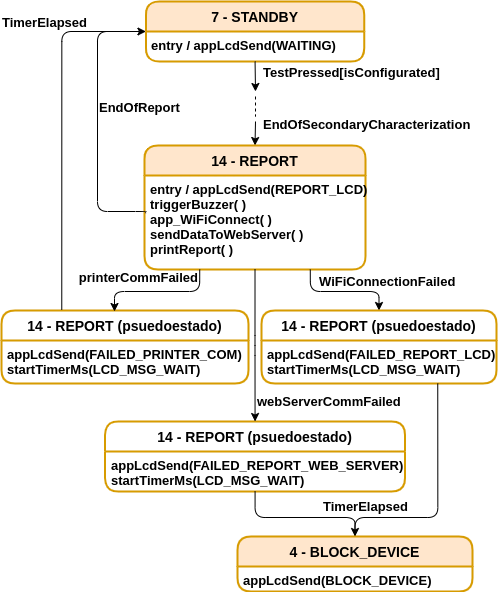
\includegraphics[scale=1]{./Figures/MainFSM_4.png}
	\caption{Etapa de reporte.}
	\label{fig:MainFSM_4}
\end{figure}

En el caso que alguno de los pasos anteriores fallen se transiciona a un pseudoestado dentro del estado \textit{REPORT} y se muestra la falla en el \textit{display}. En caso de ser una falla grave que impide la comunicación de resultados al servidor web, se transiciona al estado \textit{BLOCK\_DEVICE}.

\subsection{Medición de valor eficaz}
\label{subsec:RMS}

Los monitores de tensión y corriente de los bobinados son los bloques encargados de entregarle al controlador principal los valores RMS de dichas variables. Para tal fin, las salidas de los sensores de tensión y corriente presentados en las secciones \ref{sec:secZMPT101B} y \ref{sec:secZMCT103C} luego de pasar por un divisor resistivo acorde y un filtro pasa bajos (RC), son conectadas a cuatro canales del ADC1 del módulo ESP32-WROOM-32 como se muestra en la tabla \ref{tab:diagramaPines}.

Las rutinas encargadas de leer los valores de los canales del ADC1 y retornar dichos valores eficaces se encuentran en el archivo adc.h. En el código \ref{cod:adc_h} se muestra el archivo de cabecera simplificado. 

\begin{lstlisting}[label=cod:adc_h,caption=Pseudocódigo del módulo adc.h.] % Start your code-block

/**
 * @brief Initialize ADC 
 * 
 */
void appAdcInit(void);

/**
 * @brief Start a new RMS ADC conversion
 * 
 * @param rms
 *
 * @note This function takes about 1.6 seg in processing the four ADC channels
 *       It reads AMOUNT_OF_CYLCES cycles sampling SAMPLES_IN_20MS in 20 ms for each channel
 */
void appAdcStart(rms_t *rms);

\end{lstlisting}

En el archivo se definen dos funciones:
\begin{itemize}
\item appAdcInit que se utiliza para inicializar todo el hardware necesario para el uso del conversor analógico-digital.
\item appAdcStart que es llamada desde el controlador principal cada vez que se desea iniciar una conversión. Esta función acepta un puntero a la estructura rms\_t para devolver los valores leídos. 
\end{itemize}

Un detalle a destacar es que las funciones presentadas se documentaron por medio de Doxygen, esto es algo que se puede ver en los diferentes archivos de cabecera que se muestran a lo largo de la memoria.

En el pseudocódigo mostrado en el código \ref{cod:adc_c} se observa la implementación de la función appAdcStart. Esta función utiliza los siguientes módulos del entorno de desarrollo ESP-IDF presentados en la sección \ref{sec:ESPIDF}: 
\begin{itemize}
\item Conversor analógico-digital \citep{ADC}.
\item \textit{Inter-IC Sound} (I2S): que configurado en el modo ADC/DAC proporciona un periférico DMA para ser usado con el ADC y/o DAC \citep{I2S}.
\end{itemize}

El código presentado está simplificado para mostrar su operación pero cabe destacar que, además de lo mostrado en el código \ref{cod:adc_c}, se utilizaron diferentes herramientas de FreeRTOS en la función appAdcStart. Las colas para sincronizar el funcionamiento del DMA con el resto de la función son un ejemplo de ello.

\begin{lstlisting}[label=cod:adc_c,caption=Pseudocódigo del módulo adc.c.]

static adc_t adc[ADC_CHANNELS];

void appAdcStart(rms_t *rms) {
	int32_t s_rms;
	
	// Habilitación del DMA 
	i2s_adc_enable(I2S_NUM_0);

	// Barrido de los 4 canales del ADC1
	for (adcIndex=0; adcIndex<ADC_CHANNELS-1; adcIndex++) {		
		// Lectura del canal propiamente dicha
		i2s_read(I2S_NUM_0, buffer);
		
		// Filtro digital de primer orden
		firstOrderFilter(buffer);

		// Cálculo de valor eficaz
		adc[adcIndex].rms = getRMS(buffer);
		
		// Calibración de la entrada 
		calibration(&adc[adcIndex].rms,  adc[adcIndex].offset, adc[adcIndex].gain);
		
		// Cambiar el canal a medir del ADC1
		i2s_set_adc_mode(ADC_UNIT_1, adc[adcIndex].channel);
	}
	
	// Deshabilitar el DMA
	i2s_adc_disable(I2S_NUM_0);
}
\end{lstlisting}

Al ingresar a la función appAdcStart se habilita el DMA por medio de la función i2s\_adc\_enable. El próximo paso es barrer los cuatro canales del ADC1 para la cual se utiliza un lazo de tipo \textit{for}. Dentro del lazo la función i2s\_read muestrea el canal del ADC1 seleccionado. Dicha función fue configurada para leer 8 ciclos de la señal de entrada y tomar 128 muestras por cada ciclo, hasta que se realiza esta acción la función permanece bloqueada. Como se miden las variables de la red de energía eléctrica y su período es de 20 ms, da un tiempo de medición por canal de 160 ms, tal como se muestra en la ecuación \ref{eq:TMED}.

\begin{equation}
	\label{eq:TMED}
	T_{MED} = 8 * 20 ms = 160 ms
\end{equation}

Y se obtienen 1024 muestras por canal como se puede apreciar en la ecuación \ref{eq:puntos}.

\begin{equation}
	\label{eq:puntos}
	N = 8 * 128 = 1024
\end{equation}

Por lo tanto, la función i2s\_read permanece bloqueada durante 160 ms y devuelve un puntero a un vector con 1024 puntos de la señal de entrada. Este vector es luego filtrado con un filtro digital de primer orden cuya estructura se muestra en la ecuación \ref{eq:filtro}. Los valores de A$_{1}$ y B$_{0}$ se ajustaron convenientemente en función de la frecuencia de muestreo del sistema y la respuesta deseada del filtro.

\begin{equation}
	\label{eq:filtro}
	y\left( n \right) = A_1 y\left( n-1 \right) + B_0 x\left( n \right)
\end{equation}

Luego del filtrado se procede a calcular el valor eficaz de los valores medidos por medio de la función getRMS. Se utilizó la ecuación \ref{eq:RMS} para el cálculo del valor eficaz de las muestras obtenidas donde CICLOS=8 y N$_{CICLOS}$=128. Con el filtro digital y el promedio de 8 ciclos de la señal medida se obtiene un valor estable y ayuda a lidiar con las conexiones de la placa universal y las salidas de los módulos sensores.

\begin{equation}
	\label{eq:RMS}
rms=\frac{1}{CICLOS}\sum_{n=0}^{CICLOS-1}\sqrt{\frac{1}{N_{CICLOS}}\sum_{i=0}^{ N_{CICLOS}-1} buffer\left [ n \right ]\left [ i \right ]*buffer\left [ n \right ]\left [ i \right ]}
\end{equation}

Finalmente, se realiza una corrección lineal del valor obtenido, función calibration en el código, a partir de un desplazamiento (\textit{offset}) y una ganancia (\textit{gain}) preconfigurados. Se puede observar que cada uno de los pasos mencionados se realiza sobre cada canal independientemente, puntualmente la calibración de las señales, para la cual se cuenta con un juego de ganancias y desplazamientos independientes para cada canal.

\subsection{Comunicación Wi-Fi}

El módulo de comunicación Wi-Fi es el módulo más complejo del sistema. Este no solo debe ser capaz de controlar la configuración, conexión y desconexión del módulo a la red Wi-Fi, sino que, además, debe leer y escribir a memoria no volátil las credenciales de la red Wi-Fi y manejar el protocolo SmartConfig. 

En la figura \ref{fig:WiFi} se muestra un diagrama de flujo simplificado de las etapas seguidas para la gestión de la red Wi-Fi. 

Las principales librerías del entorno ESP-IDF utilizadas para el desarrollo de este módulo son: 
\begin{itemize}
\item \textit{Non-volatile storage library} \citep{NVL}: utilizada para leer y escribir las credenciales de Wi-Fi hacia y desde la memoria \textit{flash}. Se tuvo el cuidado de validar los datos leídos para evitar errores en las librerías de Wi-Fi por leer datos corruptos desde la memoria.
\item Wi-Fi \citep{ESPIDF:WiFi}.
\item SmartConfig: utilizado en conjunto con la aplicación móvil ESP-Touch como se explica en la sección \ref{sec:ESPTouch}.
\end{itemize}

Para sincronizar las diferentes tareas se utilizó la librería de eventos \textit{Event Loop Library} \citep{EVENT}, la cual permite pasar por los diferentes estados de la comunicación y evitar condiciones de carrera. Por simplicidad, en el diagrama de flujo de la figura \ref{fig:WiFi} se omiten estos eventos. Sin embargo, en la descripción posterior se nombrarán algunos de ellos para tener una mejor correlación con el trabajo realizado.

Para iniciar la conexión a la red Wi-Fi, el controlador principal debe llamar a la función app\_WiFiConnect como se explicó en la sección \ref{subsubsec:EtIni}. Una vez llamada dicha función ocurre la secuencia de la figura \ref{fig:WiFi}. El primer paso es leer la memoria no volátil en busca de las credenciales de Wi-Fi y en caso de obtenerlas sin error se procede a configurar el periférico en modo estación (\textit{station mode}), configurar las credenciales en una estructura de configuración provista por la librería Wi-Fi y encender el periférico. El próximo paso es esperar por el evento WIFI\_CONNECTED o el evento WIFI\_FAIL. En caso de recibir este último se reintenta 5 veces para poder conectar. Si no se logra se retorna de la función app\_WiFiConnect con el valor \textit{WiFiConnectionFailed}. En caso de obtener el evento  WIFI\_CONNECTED en alguno de los intentos la función retorna con el valor \textit{WiFiConnectionSuccessfully}.

\pagebreak

\begin{figure}[ht]
	\centering
	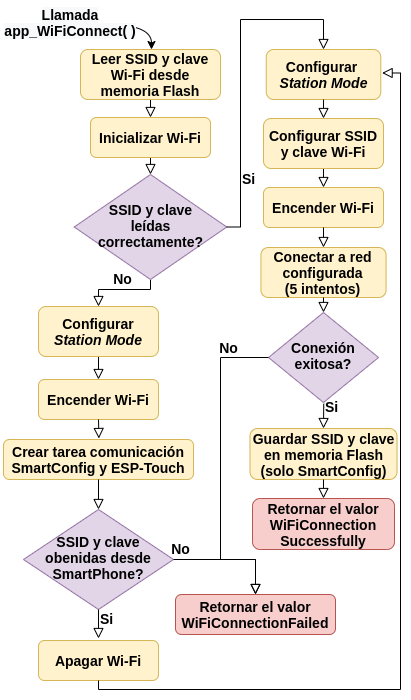
\includegraphics[scale=0.95]{./Figures/WiFi.png}
	\caption{Secuencia de conexión a red Wi-Fi.}
	\label{fig:WiFi}
\end{figure}

En caso de no tener las credenciales de Wi-Fi configuradas u obtener un error al intentar leerlas la función app\_WiFiConnect puede utilizar SmartConfig para intentar adquirirlas desde la aplicación móvil ESP-Touch. Para esto se crea una tarea de FreeRTOS para utilizar las funciones de la librería de SmartConfig. Dentro de la tarea se espera por el evento ESPTOUCH\_DONE que se genera cuando la aplicación ESP-Touch envía las credenciales. Luego de obtener las credenciales se procede a intentar conectar nuevamente por medio del procedimiento explicado en el párrafo anterior. La única diferencia en este caso es que si se logra conectar exitosamente a Wi-Fi, se guardan las nuevas credenciales en memoria no volátil para su posterior reutilización. Por otro lado, la tarea de FreeRTOS creada para administrar el protocolo SmartConfig se borra del sistema al finalizar el procedimiento ya que la acción de generar las credenciales de Wi-Fi es una tarea de un solo uso y carece de sentido tenerla corriendo todo el tiempo.


\subsection{Obtención y envío de datos al webserver}

Como se explicó en los capítulos introductorios, el cliente desarrolló un servidor web donde consultar los valores de comparación de tensiones y corrientes y a donde enviar los valores medidos y los resultados obtenidos. 

La forma de comunicarse con el servidor web es a través de comandos GET y POST de HTTP. Por otro lado, la información a ser transmitida y/o recibida se procesa en el cuerpo de los comandos GET y POST en formato JSON.

Para recibir los datos de configuración se debe enviar el siguiente comando GET:

\begin{table}[htpb]
\centering
\begin{tabular}{|l|}
\hline
\begin{tabular}[c]{@{}l@{}}\textbf{GET} /TransformersTesterConfigs/Last \textbf{http/1.1}\\ \textbf{Host:} https://iris-test-api.azurewebsites.net/api\\ \textbf{Content-Type:} application/json\end{tabular} \\ \hline
\end{tabular}
\end{table}

Y se obtiene una respuesta como la siguiente:

\begin{table}[htpb]
\centering
\begin{tabular}{|l|}
\hline
\begin{tabular}[c]{@{}l@{}}\textbf{HTTP/1.1 200 OK}\\ \textbf{Content-Type:} application/json\\ \textbf{Server:} Kestrel\end{tabular} \\ \hline
\begin{tabular}[c]{@{}l@{}}\{\\ \hspace{0.6cm}``id'':4,\\ \hspace{0.6cm}``createDate'':``2021-03-10T15:59:04'',\\ \hspace{0.6cm}``code'':``MPELETRAN-0023'',\\ \hspace{0.6cm}``batchId'':``20210310-1'',\\ \hspace{0.6cm}``vinPrimaryMin'':225.00,\\ \hspace{0.6cm}``voutSecondaryMin'':14.00,\\ \hspace{0.6cm}``iPrimaryMin'':15.00,\\ \hspace{0.6cm}``vinSecondaryMin'':14.00,\\ \hspace{0.6cm}``voutPrimaryMin'':210.00,\\ \hspace{0.6cm}``iSecondaryMin'':100.00,\\ \hspace{0.6cm}``vinPrimaryMax'':235.00,\\ \hspace{0.6cm}``voutSecondaryMax'':17.00,\\ \hspace{0.6cm}``iPrimaryMax'':70.00,\\ \hspace{0.6cm}``vinSecondaryMax'':16.00,\\ \hspace{0.6cm}``voutPrimaryMax'':230.00,\\ \hspace{0.6cm}``iSecondaryMax'':400.00\\ \}\end{tabular} \\ \hline
\end{tabular}
\end{table}

A la comunicación con el servidor web y el procesamiento de los paquetes se lo dividió en dos capas de software:
\begin{itemize}
\item Capa HTTP (http\_client.h): encargada de procesar los comandos GET y POST de HTTP.
\item Capa de procesamiento de paquetes (app\_Comm.h): encargada de tomar los datos enviados o recibidos de la capa HTTP y armar o desarmar (``parsear'') los paquetes JSON.
\end{itemize}

Para el desarrollo de la capa HTTP se utilizó la librería cliente HTTP del entorno de desarrollo ESP-IDF \citep{HTTPC}. En el código \ref{cod:http_c} se muestra un pseudocódigo para la función GET. La implementación de la función POST es similar.

\begin{lstlisting}[label=cod:http_c,caption=Pseudocódigo función GET de HTTP.]
#include "esp_http_client.h"

#define GET_URL   "https://iris-test-api.azurewebsites.net/api/TransformersTesterConfigs/Last"

esp_err_t get_http_config(char *buffer)
{
    esp_http_client_config_t config = {
    	.url = GET_URL,
    };

    // Inicializar el cliente HTTP
    esp_http_client_init(&config);
    
    // Abrir conexión con el servidor
    if ((err = esp_http_client_open(client, 0)) != ESP_OK) {
        return (err);
    }
    
    // Armar encabezado método GET
    esp_http_client_set_method(client, HTTP_METHOD_GET);
    esp_http_client_set_header(client, "Content-Type", "application/json");
    
    // Enviar paquete GET y capturar respuesta
    read_len = esp_http_client_read(client, buffer, BUFFER_SIZE);
    if (read_len <= 0) {
        return (ESP_FAIL);
    }
    
    // Cerrar la conexión con el cliente HTTP
    esp_http_client_close(client);

    return (err);
}

\end{lstlisting}

En el caso de un comando GET los datos recibidos desde la capa HTTP son luego pasados a la capa de procesamiento de paquetes donde se procede a ``parsearlos'' y validarlos. Entre las rutinas de validación se encuentra el chequeo de los datos numéricos. En la capa de procesamiento los datos se guardan en una estructura de tipo configData\_t diseñada para tal fin. La estructura configData\_t permite el fácil acceso de los datos obtenidos del servidor web por parte del controlador principal. En el código \ref{cod:struct_http} se muestra la jerarquía de estructuras desarrollada para la estructura configData\_t, aquí también se puede apreciar que está documentada con Doxygen.

\begin{lstlisting}[label=cod:struct_http,caption=Estructuras para el manejo de los datos recibidos.]
/**
 * @brief Parameter thresholds structure
 *
 */
typedef struct {
	int32_t max;
	int32_t min;
} parametersRange_t;

/**
 * @brief Measured Parameters structure
 *
 */
typedef struct {
	parametersRange_t Vinp;   /*!<Primary Voltage    */
	parametersRange_t Voutp;  /*!<Primary Voltage    */
	parametersRange_t Vins;   /*!<Secondary Voltage  */
	parametersRange_t Vouts;  /*!<Secondary Voltage  */
	parametersRange_t Ip;     /*!<Primary current    */
	parametersRange_t Is;     /*!<Secondary current  */
} trafoParameters_t;

/**
 * @brief Configuration data type
 *
 */
typedef struct {
	uint32_t id;                      /*!<Test Identification Number   */
	char batchId[BATCHID_LENGTH];     /*!<Transformer BatchId          */
	char code[CODE_LENGTH];           /*!<Transformer code             */
	trafoParameters_t trafoParameters;/*!<Measured Parameters structure*/
} configData_t;
\end{lstlisting}


\subsection{Implementación del protocolo DPL}

Entre las tareas que el controlador principal debe realizar en la etapa de reporte (sección \ref{subsubsec:EtRep}) se encuentra la impresión de una etiqueta con los resultados del ensayo. Para ello se utilizó la impresora presentada en la sección \ref{sec:Impre} cuyo protocolo se conoce como DPL y fue introducido en la misma sección. En esta sección se explica la implementación de dicho protocolo.

El protocolo DPL fue implementado en el módulo app\_printer.c, en tanto que la capa física del protocolo fue resuelta con el módulo de hardware presentado en la sección \ref{fig:rs232}. Para su manejo se utilizó la librería UART que se encuentra dentro de los controladores de periféricos provistos por el entorno ESP-IDF \citep{ESPIDF:PER}.

Cuando el controlador principal desea imprimir los resultados del ensayo debe llamar a la función \textit{print}. Esta función implementa todos los comandos necesarios para utilizar el protocolo DPL y devuelve el resultado de la impresión. En el código \ref{cod:print_h} se muestran los valores devueltos por la función \textit{print}.

 \begin{lstlisting}[label=cod:print_h,caption=Prototipo función print.]
/**
 * @brief Printer status
 * 
 */
typedef enum {
	PRINTER_NO_COMM,   /*!<Printer never respond             */
	PRINTER_NOT_READY, /*!<Printer is not ready, answer to 
	                       command <SOH>A/r (Status request) */
	PRINTER_READY,     /*!<Printer ready to print            */
	PRINTER_OK         /*!<The print command was successful  */
} printerStatus_t;
\end{lstlisting}

En la figura \ref{fig:printFunc} se muestra el diagrama de flujo de la función \textit{print}. Los comandos a enviar y la respuesta de la impresora se resaltan en color azul, mientras que el contenido de la etiqueta (resultado obtenido del ensayo y valores medidos) se resalta en verde.

\pagebreak

\begin{figure}[htpb]
	\centering
	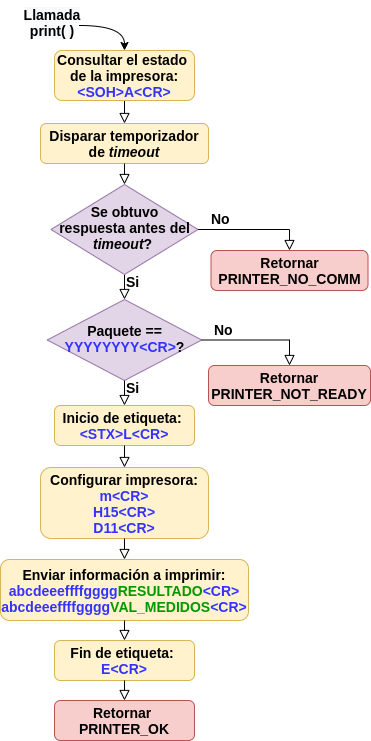
\includegraphics[scale=0.95]{./Figures/printer.png}
	\caption{Diagrama de flujo función de la \textit{print}.}
	\label{fig:printFunc}
\end{figure}

La primera acción a realizar al llamar la función \textit{print} es verificar el estado de la impresora. Para ello se envía el comando inmediato \textless{}SOH\textgreater{}A\textless{}CR\textgreater{} y a su vez, se dispara un temporizador de espera (\textit{timeout}). Si el temporizador de espera llega a su valor de temporización antes que la impresora haya respondido, la función retorna un error de comunicación con la impresora (PRINTER\_NO\_COMM). En caso de recibir una  respuesta en el tiempo estipulado, esta es analizada y si es igual a la cadena ``YYYYYYYY\textless{}CR\textgreater{}'' significa que la impresora está en condiciones de imprimir. Por otro lado, en caso de recibir algún carácter 'N' dentro de la trama anterior significa que la impresora no está disponible y se retorna de la función \textit{print} con un estado de error PRINTER\_NOT\_READY.

En caso que la impresora esté en condiciones de imprimir (PRINTER\_READY) se pasa a enviar el comando \textless{}STX\textgreater{}L\textless{}CR\textgreater{} para iniciar la impresión de la etiqueta propiamente dicha. Después de este, se envían los siguientes comandos de configuración propios de la etiqueta en cuestión:
\begin{itemize}
\item m\textless{}CR\textgreater{}: indica que la etiqueta utiliza unidades internacionales.
\item H15\textless{}CR\textgreater{}: fija la temperatura del cabezal de impresión.
\item D11\textless{}CR\textgreater{}: fija el tamaño del punto de impresión.
\end{itemize}

Una vez configurada la impresora para la etiqueta en particular se procede a enviar la información a imprimir por medio del formato presentado en la tabla \ref{tab:printercmdSystem}. En la figura se indican genéricamente los caracteres ``abcdeeeffffgggg'' ya que estos dependen de cada línea que se quiera imprimir (rotación del texto, tipo de fuente, ubicación del texto, etc). En la misma línea y luego de los caracteres mencionados se encuentra el dato a imprimir que depende del ensayo (RESULTADO y VAL\_MEDIDOS).

Por último, se envía el comando E\textless{}CR\textgreater{} que le indica a la impresora que se finalizó la carga de la etiqueta y se puede proceder a su impresión. Si se llega al final de este proceso la función \textit{print} devuelve PRINTER\_OK que significa que se pudo imprimir con éxito.

\subsection{Interfaz de usuario}

La interfaz local de usuario está formada por los siguientes elementos:
\begin{itemize}
\item Pulsadores Testear, Configurar y Cancelar.
\item \textit{Buzzer}.
\item \textit{Display} alfanumérico de 20 caracteres por 4 líneas.
\end{itemize}

Para trabajar con todos estos módulos se utilizó la librería GPIO que se encuentra dentro de los controladores de periféricos provistos por el entorno ESP-IDF \citep{ESPIDF:PER}.

Para el procesamiento de los pulsadores se desarrolló una función para cada uno. Estas funciones deben ser encuestadas (\textit{pulling}) periódicamente para saber el estado de los pulsadores. En el código \ref{cod:app_gpio_h} se muestra el prototipo para el pulsador Cancelar. Adicionalmente, se incorporaron rutinas antirebote (\textit{debouncing}) para todos los pulsadores.

\begin{lstlisting}[label=cod:app_gpio_h,caption=Prototipo para el pulsador Cancelar.]
/**
 * @brief Check if the cancel button was pressed
 * 
 * @return true 
 * @return false 
 */
bool isCancelPressed( void );
\end{lstlisting}

En caso del accionamiento del \textit{buzzer} se deben generar 2 secuencias según el requerimiento 3 de la sección \ref{subsec:ReqUsu}, para lo cual se utiliza un temporizador de hardware. Para la implementación del temporizador se usó la librería de temporizadores provista por el entorno ESP-IDF dentro de los controladores de periféricos \citep{ESPIDF:PER}.

Por último, para el \textit{display} se tomó como base la librería sAPI \citep{sAPI} que posee un módulo de software para utilizar el controlador HD44780. El código debió ser portado para funcionar en el entorno ESP-IDF. Además del trabajo anterior, se trabajó en mejorar la librería de la sAPI por medio del agregado de varias estructuras de software que permiten inicializar el controlador del \textit{display} de una manera más eficiente.

